\documentclass[12pt]{eskdtext}
\usepackage[numbertop, numbercenter]{eskdplain}
\usepackage[utf8x]{inputenc}

% - Подключаем шрифты из пакета scalable-cyrfonts-tex
\usepackage{cyrtimes}

% - Отступ красной строки
\setlength{\parindent}{1.25cm}

% - Убирает точку в списке литературы
\makeatletter
\def\@biblabel#1{#1 }

% - Точки для всех пунктов в оглавлении
\renewcommand*{\l@section}{\@dottedtocline{1}{1.5em}{2.3em}}
\renewcommand*{\l@subsection}{\@dottedtocline{1}{1.5em}{2.3em}}
\renewcommand*{\l@subsubsection}{\@dottedtocline{1}{1.5em}{2.3em}}

% - Для переопределения списков
\renewcommand{\theenumi}{\arabic{enumi}}
\renewcommand{\labelenumi}{\theenumi)}
\makeatother

\usepackage{enumitem}
\setlist{nolistsep, itemsep=0.3cm,parsep=0pt}

% - ГОСТ списка литературы
\bibliographystyle{utf8gost705u}

% - Верикальные отступы заголовков 
\ESKDsectSkip{section}{1em}{1em}
\ESKDsectSkip{subsection}{1em}{1em}
\ESKDsectSkip{subsubsection}{1em}{1em}

% - Изменение заголовков
\usepackage{titlesec}
\titleformat{\section}{\centering\normalfont\normalsize}{\thesection}{1.0em}{}
\titleformat{\subsection}{\centering\normalfont\normalsize}{\thesubsection}{1.0em}{}
\titleformat{\subsubsection}{\centering\normalfont\normalsize}{\thesubsubsection}{1.0em}{}
\titleformat{\paragraph}{\centering\normalsize}{\theparagraph}{1.0em}{}

% - Оставим место под ТЗ 
%\setcounter{page}{4}

% - Для больших таблиц
\usepackage{longtable}
\usepackage{tabularx}
\renewcommand{\thetable}{\thesection.\arabic{table}}

% - Используем графику в документе
\usepackage{graphicx}
\graphicspath{{images/}}
\renewcommand{\thefigure}{\thesection.\arabic{figure}}

% - Счётчики
\usepackage{eskdtotal}

% - Выравнивание по ширине
\sloppy

% - Разрешить перенос двух последних букв слова
\righthyphenmin=2

\RequirePackage{enumitem}
\renewcommand{\alph}[1]{\asbuk{#1}}
\setlist{nolistsep}
\setitemize[1]{label=--, fullwidth, itemindent=\parindent, 
  listparindent=\parindent}% для дефисного списка
\setenumerate[1]{label=\arabic*), fullwidth, itemindent=\parindent, 
  listparindent=\parindent}% для нумерованного списка
\setenumerate[2]{label=\alph*), fullwidth, itemindent=\parindent, 
  listparindent=\parindent, leftmargin=\parindent}% для списка 2-ой ступени, который будет нумероваться а), б) и т.д.

% - Оформляем листинг кода (не использовать комментарии на русском!)
\usepackage{listings}  
\lstset{basicstyle=\ttfamily\small}
\lstset{extendedchars=\true}

% - выводим текст как есть с размером шрифта scriptsize
\makeatletter
\def\verbatim{\scriptsize\@verbatim \frenchspacing\@vobeyspaces \@xverbatim}
\makeatother


\begin{document}
 \newpage
\ESKDthisStyle{empty}

\begin{center}
 Министерство образования и науки Российской Федерации\\
 Федеральное государственное бюджетное образовательное учреждение высшего профессионального образования\\
 <<ТОМСКИЙ ГОСУДАРСТВЕННЫЙ УНИВЕРСИТЕТ СИСТЕМ УПРАВЛЕНИЯ И РАДИОЭЛЕКТРОНИКИ>> (ТУСУР)\\
 Кафедра комплексной информационной безопасности электронно-вычислительных систем (КИБЭВС)\\
\end{center}

\vfill

\begin{flushright}
\begin{minipage}{0.45\textwidth}
 \begin{flushleft}
  УТВЕРЖДАЮ\\
  заведующий каф. КИБЭВС
  \underline{\hspace{3cm}}А.А. Шелупанов \\
  <<\underline{\hspace{1cm}}>>\underline{\hspace{3cm}}2016г.\\
 \end{flushleft}
\end{minipage}
\end{flushright}

\vfill

\begin{center}
ПРОГРАММНЫЙ КОМПЛЕКС ДЛЯ ПРОВЕДЕНИЯ СОРЕВНОВАНИЙ В ОБЛАСТИ ИНФОРМАЦИОННОЙ БЕЗОПАСНОСТИ

Отчет по групповому проектному обучению

Группа КИБЭВС-1502
\end{center}

\vfill
\begin{flushright}
\begin{minipage}{0.45\textwidth}
 \begin{flushleft}
  Ответственный исполнитель \\
  студент гр. 723 \\
  \underline{\hspace{3cm}}Д.Е. Муковкин \\
  <<\underline{\hspace{1cm}}>>\underline{\hspace{3cm}}2016г.\\
 \end{flushleft}
\end{minipage}
\end{flushright}

\vfill

\begin{flushright}
\begin{minipage}{0.45\textwidth}
 \begin{flushleft}
  Научный руководитель \\
  аспирант каф. КИБЭВС \\
  \underline{\hspace{3cm}}А.И. Гуляев \\
  <<\underline{\hspace{1cm}}>>\underline{\hspace{3cm}}2016г.\\
 \end{flushleft}
\end{minipage}
\end{flushright}

\vfill

\begin{center}
 2016
\end{center}

 \newpage
\ESKDthisStyle{empty}
\paragraph{\hfill РЕФЕРАТ \hfill}
Курсовая работа содержит \ESKDtotal{page} страниц, \ESKDtotal{figure} рисунка, \ESKDtotal{table} таблицы, \ESKDtotal{bibitem} источников, \ESKDtotal{appendix} приложение.

%допилить ключевые слова
КОМПЬЮТЕРНАЯ ЭКСПЕРТИЗА, ФОРЕНЗИКА, ЛОГИ, QT, XML, GIT, LATEX, MOZILLA THUNDERBIRD, MS OUTLOOK, WINDOWS, PST, MSG, RTF, HTML, БИБЛИОТЕКИ, РЕПОЗИТОРИЙ, ПОЧТОВЫЙ КЛИЕНТ, SQLLITE, РЕЕСТР, МЕТА-ДАННЫЕ, READPST, JPEG, PNG, ID3V1, JFIF, RIFF, CHUNK, DBX, C++, DOXYGEN.

Цель работы --- создание программного комплекса, предназначенного для проведения компьютерной экспертизы.

Задачей, поставленной на данный семестр, стало написание программного комплекса, имеющего следующие возможности: 
\begin{enumerate}
\item сбор и анализ информации из журналов истории браузеров;
\item сбор и анализ информации из мессенджеров;
\item сбор и анализ информации из почтовых приложений;
\item поиск медиа-файлов (аудио, видео, изображение) и извлечение мета-данных из них;
\item сбора информации об установленном ПО по остаточным файлам.
\item сбор и анализ информации из реестра Windows.
\end{enumerate}

Результаты работы в данном семестре:

\begin{itemize}
\item реализован импорт истории посещений, поисковых запросов, загруженных файлов, списка установленных расширений, информации о версии программы и подключенном аккаунтеGoogle из приложения Google Chrome;
\item реализован алгоритм сканирования директорий ОС Windows на содержание файлов, оставшихся при установке или после удаления различных программ;
\item реализован алгоритм извлечения адресата, отправителя, темы, даты и текста
сообщения из файлов формата <<.dbx>>, используемого MS Outlook для хранения сообщений;
\item реализован алгоритм извлечения времени, даты, отправителя, получателя и текст
сообщения почтового клиента Mozilla Thunderbird;
\item реализован алгоритм извлечения мета-данных из фалов формата ID3v1, JFIF и RIFF;
\item реализован алгоритм извлечения информации из реестра Windows (.reg-файлов).
\end{itemize}

Пояснительная записка выполнена при помощи системы компьютерной вёрстки \LaTeX.

 
 \newpage
 \ESKDthisStyle{empty}
 \section*{Список исполнителей}
 
Лобанов О.В. -- программист, ответственный исполнитель, ответственный за разработку функций сбора информации из реестра. 

Шиповской В.В. -- программист, ответственный за написание части системы для сбора и обработки информации из браузера Google Chrome.

Серяков А.В. -- программист, ответственный за написание части системы для сбора информации из почтового клиента MS Outlook.

Боков И.М. -- программист, ответственный за написание части системы для для нахождения медиа-файлов (аудио, видео, изображение) и извлечения мета-данных из них.

Кучер М.В. -- программист, ответственный за написание части системы для сбора информации об установленном ПО по остаточным файлам.

Терещенко Ю.А. -- программист, ответственный за написание части системы для сбора информации из почтового клиента Mozilla Thunderbird.

Мейта М.В. -- документатор, ответсвенный за верстку необходимой документации в системе \LaTeX.

 
 % - содержание
 \newpage
 \ESKDstyle{plain}
 \tableofcontents

 \newpage
 \ESKDstyle{plain}
 \section*{Введение}
 \addcontentsline{toc}{section}{Введение}
 CTF (Capture the flag, Захват флага) - это командные соревнования, целью которых является оценка умения участников атаковать и защищать компьютерные системы. По типу, соревнования делятся на два типа: task-based (квесты), attack-defense (классические соревнования).

Для проведения соревнований типа attack-defense, каждой команде выдается сервер, на котором имеется ряд сервисов, одинаковые у всех. Сервисами являются программы, которые должны быть запущены на протяжении всего времени соревнований. Раз в минуту жюрейская система проверяет работу сервисов, присылает новый флаг, а также проверяет его наличие на сервере. В роли флага выступает случайно сгенерированная строка, определенной длины. Сервисы заведомо имеют уязвимости, через которые можно украсть флаг. Команда должна найти уязвимости в сервисах и закрыть их. Но также она должна эксплуатировать эти уязвимости на сервисах других команд, похищая флаги. 

Команда Keva имеет большой опыт в проведении соревнований CTF. Во время проведения межрегиональных межвузовских соревнований в области информационной безопасности SibirCTF 2014, 2015 использовались наработки Екатеринбургской команды HackerDom. Однако их решение не подходит нам по некоторым критически важным параметрам. Поэтому  было принято решение написать собственную платформу для проведения соревнований CTF.

Платформа должна отвечать следующим требованиям:
\begin{itemize}
\item Низкое потребление ресурсов сервера;
\item Управление игрой через графический интерфейс;
\item Возможность горизонтального масштабирования.
\end{itemize}

При разработке платформы должны быть использованы уже имеющиеся наработки, в частности, панель администратора и API для task-based проведения соревнований. 

Новая платформа позволит проводить собственные соревнования не используя готовые решения. 


 \section{Назначение и область применения}
Разрабатываемый комплекс предназначен для автоматизации процесса сбора информации с исследуемого образа жёсткого диска.
\section{Постановка задачи}
\setcounter{figure}{0}
В данной курсовой работе были поставлены следующие задачи:

\begin{itemize}
\item выбор инструментов разработки платформы;
\item разработка архитектуры;
\item определение индивидуальных задач для каждого участника проектной группы;
\item исследование предметных областей в рамках индивидуальных задач;
\item реализация новых программных модулей и доработка уже существующих.
\end{itemize}

Задачи, связанные с разработкой программного комплекса:

\begin{enumerate}
\item разработка ядра платформы;
\item разработка модуля проверяющей системы;
\item разработка модуля сдачи флага;
\item разработка модуля рейтинговой таблицы;
\item доработка модуля администраторской панели.
\end{enumerate}

Задачи, связанные с тестированием программного комплекса:

\begin{enumerate}
\item проверка работы ядра;
\item проверка работы модуля проверяющей системы;
\item проверка работы модуля сдачи флага;
\item проверка работы модуля рейтинговой таблицы;
\item проверка работы модуля администраторской панели.
\end{enumerate}

\section{Инструменты}
\setcounter{figure}{0}
\subsection{Система контроля версий Git}
Для разработки программного комплекса для проведения компьютерной экспертизы было решено использовать Git.

Git --- распределённая система управления версиями файлов. Проект был создан Линусом Торвальдсом для управления разработкой ядра Linux  как противоположность  системе управления версиями Subversion (также известная как «SVN») \cite{progit}.

При работе над одним проектом команде разработчикоа необходим инструмент для совместного написания, бэкапирования и тестирования программного обеспечения. Используя Git, мы имеем:
\begin{itemize}
\item возможность удаленной работы с исходными кодами;
\item возможность создавать свои ветки, не мешая при этом другим разработчикам;
\item доступ к последним изменениям в коде, т.к. все исходники хранятся на сервере git.keva.su;
\item исходные коды защищены, доступ к ним можно получить лишь имея RSA-ключ;
\item возможность откатиться к любой стабильной стадии проекта.
\end{itemize}

Основные постулаты работы с кодом в системе Git:

\begin{itemize}
\item каждая задача решается в своей ветке;
\item необходимо делать коммит как только был получен осмысленный результат;
\item ветка master мержится не разработчиком, а вторым человеком, который производит вычитку и тестирование изменения;
\item все коммиты должны быть осмысленно подписаны/прокомментированы.
\end{itemize}

Для работы над проектом проектной группой был поднят собственный репозиторий на сервере git.keva.su.
Адреса репозиториев следующие:

Исходные файлы проекта:

git clone git@git.keva.su:gpo.git gpo.git

Репозиторий для тестирования проекта:

git clone git@git.keva.su:gpo-testdata.git gpo-testdata.git

\subsection{Система компьютерной вёрстки \TeX}
\TeX\ --- это созданная американским математиком и программистом Дональдом Кнутом система для вёрстки текстов. Сам по себе \TeX\ представляет собой специализированный язык программирования.Каждая издательская система представляет собой пакет макроопределений этого языка.

\LaTeX\ --- это созданная Лэсли Лэмпортом издательская система на базе \TeX'а\cite{lvovskyi}. \LaTeX\ позволяет пользователю сконцентрировать свои услия на содержании и структуре текста, не заботясь о деталях его оформления.

Для подготовки отчётной и иной документации нами был выбран \LaTeX\, так как совместно с системой контроля версий Git он предоставляет возможность совместного создания и редактирования документов. Огромным достоинством системы \LaTeX\ то, что создаваемые с её помощью файлы обладают высокой степенью переносимости \cite{latexrus}.

Совместно с \LaTeX\ часто используется Bib\TeX\ --- программное обеспечение для создания форматированных списков библиографии. Оно входит в состав дистрибутива \LaTeX\ и позволяет создавать удобную, универсальную и долговечную библиографию. Bib\TeX\ стал одной из причин, по которой нами был выбран \LaTeX\ для создания документации.

\subsection{Система документирования Doxygen}
Doxygen --- это кроссплатформенная система документирования исходных текстов, которая поддерживает разлличные языки программирования (в том числе и C++) \cite{doxygen}. 

Doxygen генерирует документацию на основе набора исходных текстов и также может быть настроен для извлечения структуры программы из недокументированных исходных кодов. Возможно составление графов зависимостей программных объектов, диаграмм классов и исходных кодов с гиперссылками.

Doxygen имеет встроенную поддержку генерации документации в формате HTML, \LaTeX\, man, RTF и XML. Также вывод может быть легко сконвертирован в CHM, PostScript, PDF.

Doxygen — консольная программа в духе классической Unix. Она работает подобно компилятору, анализируя исходные тексты и создавая документацию. Параметры создания документации читаются из конфигурационного файла, имеющего простой текстовый формат.

Автором программы является голландец Димитри ван Хееш (Dimitri van Heesch).

QT Creator --- среда разработки, использумая разработчиками coex --- поддерживает формат комментариев, используемого Doxygen при генерации документации. В ходе работы была сгенерирована документация при помощи данного инструмента, представляющая собой набор связанных html-страниц, описывающих различные классы и функции, используемые в coex. В дальнейшем планируется усовершенствовать полученную документацию, добавить описания для всех программных объектов.

\subsection{Qt - кроссплатформенный инструментарий разработки ПО}
Qt --- это кроссплатформенная библиотека C++ классов для создания графических пользовательских интерфейсов (GUI) от фирмы Digia. Эта библиотека полностью объектно-ориентированная, что обеспечивает легкое расширение возможностей и создание новых компонентов. Ко всему прочему, она поддерживает огромнейшее количество платформ.

Qt позволяет запускать написанное с его помощью ПО в большинстве современных операционных систем путём простой компиляции программы для каждой ОС без изменения исходного кода. Включает в себя все основные классы, которые могут потребоваться при разработке прикладного программного обеспечения, начиная от элементов графического интерфейса и заканчивая классами для работы с сетью, базами данных и XML. Qt является полностью объектно-ориентированным, легко расширяемым и поддерживающим технику компонентного программирования.

Список использованных классов фраемворка QT
\begin{itemize}
\item iostream
\item QChar
\item QCryptographicHash
\item QDateTime
\item QDir
\item QDirIterator
\item QFile
\item QFileInfo
\item QIODevice
\item QList
\item QRegExp
\item QString
\item QTextStream
\item QtSql/QSqlDatabase
\item QVector
\item QMap
\item QXmlStreamReader
\item QXmlStreamWriter
\item Conversations
\end{itemize}

Класс QXmlStreamWriter представляет собой XML писателя с простым потоковым.

Класс QXmlStreamReader представляет собой быстрый синтаксически корректный XML анализатор с простым потоковым API. 

QVector представляет собой класс для создания динамических массивов.

Модуль QtSql/QSqlDatabase помогает обеспечить однородную интеграцию БД в ваши Qt приложения.

Класс QTextStream предоставляет удобный интерфейс для чтения и записи текста.

QTextStream может взаимодействовать с QIODevice, QByteArray или QString. Используя потоковые операторы QTextStream, вы можете легко читать и записывать слова, строки и числа. При формировании текста QTextStream поддерживает параметры форматирования для заполнения и выравнивания полей и форматирования чисел. \cite{qtdoc}

Класс QString предоставляет строку символов Unicode.

Класс QMap --- контейнерный класс для хранения элементов различных типов данных.

Класс QDateTime используется для работы с форматом даты, в который записывается информация о файле.

QString хранит строку 16-битных QChar, где каждому QChar соответствует один символ Unicode 4.0. (Символы Unicode со значениями кодов больше 65535 хранятся с использованием суррогатных пар, т.е. двух последовательных QChar.)

Unicode - это международный стандарт, который поддерживает большинство использующихся сегодня систем письменности. Это расширение US-ASCII (ANSI X3.4-1986) и Latin-1 (ISO 8859-1), где все символы US-ASCII/Latin-1 доступны на позициях с тем же кодом.

Внутри QString использует неявное совместное использование данных (копирование-при-записи), чтобы уменьшить использование памяти и избежать ненужного копирования данных. Это также позволяет снизить накладные расходы, свойственные хранению 16-битных символов вместо 8-битных.

В дополнение к QString Qt также предоставляет класс QByteArray для хранения сырых байт и традиционных нультерминальных строк. В большинстве случаев QString - необходимый для использования класс. Он используется во всем API Qt, а поддержка Unicode гарантирует, что ваши приложения можно будет легко перевести на другой язык, если в какой-то момент вы захотите увеличить их рынок распространения. Два основных случая, когда уместно использование QByteArray: когда вам необходимо хранить сырые двоичные данные и когда критично использование памяти (например, в Qt для встраиваемых Linux-систем).\cite{qtcross}

Класс QRegExp предоставляет сопоставление с образцом при помощи регулярных выражений.

Регулярное выражение, или ''regexp'', представляет собой образец для поиска соответствующей подстроки в тексте. Это полезно во многих ситуациях, например:

Проверка правильности -- регулярное выражение может проверить, соответствует ли подстрока каким-либо критериям, например, целое ли она число или не содержит ли пробелов.
Поиск -- регулярное выражение предоставляет более мощные шаблоны, чем простое соответствие строки, например, соответствие одному из слов mail, letter или correspondence, но не словам email, mailman, mailer, letterbox и т.д.
Поиск и замена -- регулярное выражение может заменить все вхождения подстроки другой подстрокой, например, заменить все вхождения \& на \&amp;, исключая случаи, когда за \& уже следует amp;.
Разделение строки -- регулярное выражение может быть использовано для определения того, где строка должна быть разделена на части, например, разделяя строку по символам табуляции.

QFileInfo  - Во время поиска возвращает полную информацию о файле.

Класс QDir обеспечивает доступ к структуре каталогов и их содержимого.

QIODevice представляет собой базовый класс всех устройств ввода/вывода в Qt.

Класс QCryptographicHash предоставляет способ генерации криптографических хэшей.
QCryptographicHash могут быть использованы для генерации криптографических хэшей двоичных или текстовых данных.В настоящее время MD4, MD5, и SHA-1 поддерживаются.\cite{qtcross}

QChar обеспечивает поддержку 16-битных символов Unicode.

\subsubsection{Aвтоматизация поиска журнальных файлов}

Для сканирования образа на наличие интересующих лог файлов использовался класс QDirIterator. После вызова происходит поочередный обход по каждому файлу в директории и поддиректории. Проверка полученного полного пути к файлу осуществляется регулярным выражением, если условие выполняется, происходит добавление в список обрабатываемых файлов.

\subsubsection{Реализация сохранения результатов работы программного комплекса в XML}

Cохранение полученных данных происходит в ранее выбранный формат XML(Extensible Markup Language). Для этого используется класс QXmlStreamReader и QxmlStreamWriter.
Класс QXmlStreamWriter представляет XML писателя с простым потоковым API.

QXmlStreamWriter работает в связке с QXmlStreamReader для записи XML. Как и связанный класс, он работает с QIODevice, определённым с помощью setDevice().

Сохранение данных реализованно в классе WriteMessage. В методе WriteMessages, структура которого представлена на UML диаграмме в разделе Архитектура.

\subsection{База данных MongoDB}
Для реализации программного комплекса для проведения соревнований в области информационной безопасноти была использована база данных MongoDB.

MongoDB --- документо-ориентированная система управления базами данных (СУБД) с открытым исходным кодом, не требующая описания схемы таблиц. Написана на языке C++. \cite{mongo}.

Основные возможности MongoDB:
\begin{itemize}
\item Документо-ориентированное хранение (JSON-подобная схема данных);
\item Достаточно гибкий язык для формирования запросов;
\item Динамические запросы;
\item Поддержка индексов;
\item Профилирование запросов;
\item Быстрые обновления «на месте»;
\item Эффективное хранение двоичных данных больших объёмов, например, фото и видео;
\item Журналирование операций, модифицирующих данные в базе данных;
\item Поддержка отказоустойчивости и масштабируемости: асинхронная репликация, набор реплик и распределения базы данных на узлы;
\item Возможность работы в соответствии с парадигмой MapReduce;
\item Полнотекстовый поиск, в том числе на русском языке, с поддержкой морфологии.
\end{itemize}

Архитектура:

СУБД управляет наборами JSON-подобных документов, хранимых в двоичном виде в формате BSON. Хранение и поиск файлов в MongoDB происходит благодаря вызовам протокола GridFS. Подобно другим документо-ориентированным СУБД (CouchDB и др.), MongoDB не является реляционной СУБД. В СУБД:

\begin{itemize}
\item Нет такого понятия, как «транзакция». Атомарность гарантируется только на уровне целого документа, то есть частичного обновления документа произойти не может;
\item Отсутствует понятие «изоляции». Любые данные, которые считываются одним клиентом, могут параллельно изменяться другим клиентом.
\end{itemize}

В MongoDB реализована асинхронная репликация в конфигурации «ведущий — ведомый» (англ. master — slave), основанная на передаче журнала изменений с ведущего узла на ведомые. Поддерживается автоматическое восстановление в случае выхода из строя ведущего узла. Серверы с запущенным процессом mongod должны образовать кворум, чтобы произошло автоматическое определение нового ведущего узла. Таким образом, если не используется специальный процесс-арбитр (процесс mongod, только участвующий в установке кворума, но не хранящий никаких данных), количество запущенных реплик должно быть нечётным.


\section{Технические характеристики}
\subsection {Требования к аппаратному обеспечению}

Необходимо 2 и более компьютера, находящихся в локальной сети.

Минимальные системные требования:

\begin{itemize}
\item процессор 1ГГц Pentium 4;
\item оперативная память 512 Мб;
\item место на жёстком диске -- 9 Гб.
\end{itemize}

\subsection {Требования к программному обеспечению}
Для корректной работы разрабатываемого программного комплекса на компьютере должны быть установлены пакеты: Python 3.X, MongoDB. 

\subsection{Выбор единого формата выходных файлов}
Для вывода результата был выбран формат XML-документов, так как с данным форматом лего работать при помощи программ, а результат работы данного комплекса в дальнейшем планируется обрабатывать при помощи программ.

XML - eXtensible Markup Language или расширяемый язык разметки. Язык XML представляет собой простой и гибкий текстовый формат, подходящий в качестве основы для создания новых языков разметки, которые могут использоваться в публикации документов и обмене данными \cite{xml}. Задумка языка в том, что он позволяет дополнять данные метаданными, которые разделяют документ на объекты с атрибутами. Это позволяет упростить программную обработку документов, так как структурирует информацию.

Простейший XML-документ может выглядеть так:


\begin{verbatim}
<?xml version="1.0"?>
<list_of_items>
<item id="1"\><first/>Первый</item\>
<item id="2"\>Второй <subsub_item\>подпункт 1</subsub_item\></item\>
<item id="3"\>Третий</item\>
<item id="4"\><last/\>Последний</item\>
</list_of_items>
\end{verbatim}


Первая строка - это объявление начала XML-документа, дальше идут элементы документа <list\_of\_items> - тег описывающий начало элемента \\list\_of\_items, </list\_of\_items> - тег конца элемента. Между этими тегами заключается описание элемента, которое может содержать текстовую информацию или другие элементы (как в нашем примере). Внутри тега начала элемента так же могут указывать атрибуты элемента, как например атрибут id элемента item, атрибуту должно быть присвоено определенное значение.


\section{Разработка программного обеспечения}
\setcounter{figure}{0}
 
\subsection{Архитектура}
\subsubsection{Основной алгоритм}
В ходе разарботки был применен видоизменнённый шаблон проектирования Factory method.


\subsection{Модуль: прием и проверка принятых флагов} % - Отчёт flags
В соревнованиях по информационной безопасности задача команд найти уязвимость и эксплуатировать её, добывая секретную информацию, в нашем случае флаги. Целью модуля является прием и проверка на валидность флагов.

\subsubsection{Принцип работы}

Программа реализована с использованием вебсокетов. На порту, полученном с API, программа сравнивает IP адрес клиента с данными в базе данных и при нахождении его, клиент определяется как одна из команд и может отправить серверу строку. Строка проверяется на длину символов. Так же флаг проверяется на наличие в базе данных, времени его жизни (флаги валидны определенное количество времени), принадлежность другой команде (свои флаги сдавать нельзя) и статус сервиса (аналогичный сервис сдающей команды должен быть поднят). 

Ниже представлен алгоритм и наглядная схема работы flags.py

\begin{figure}[h!]
\center{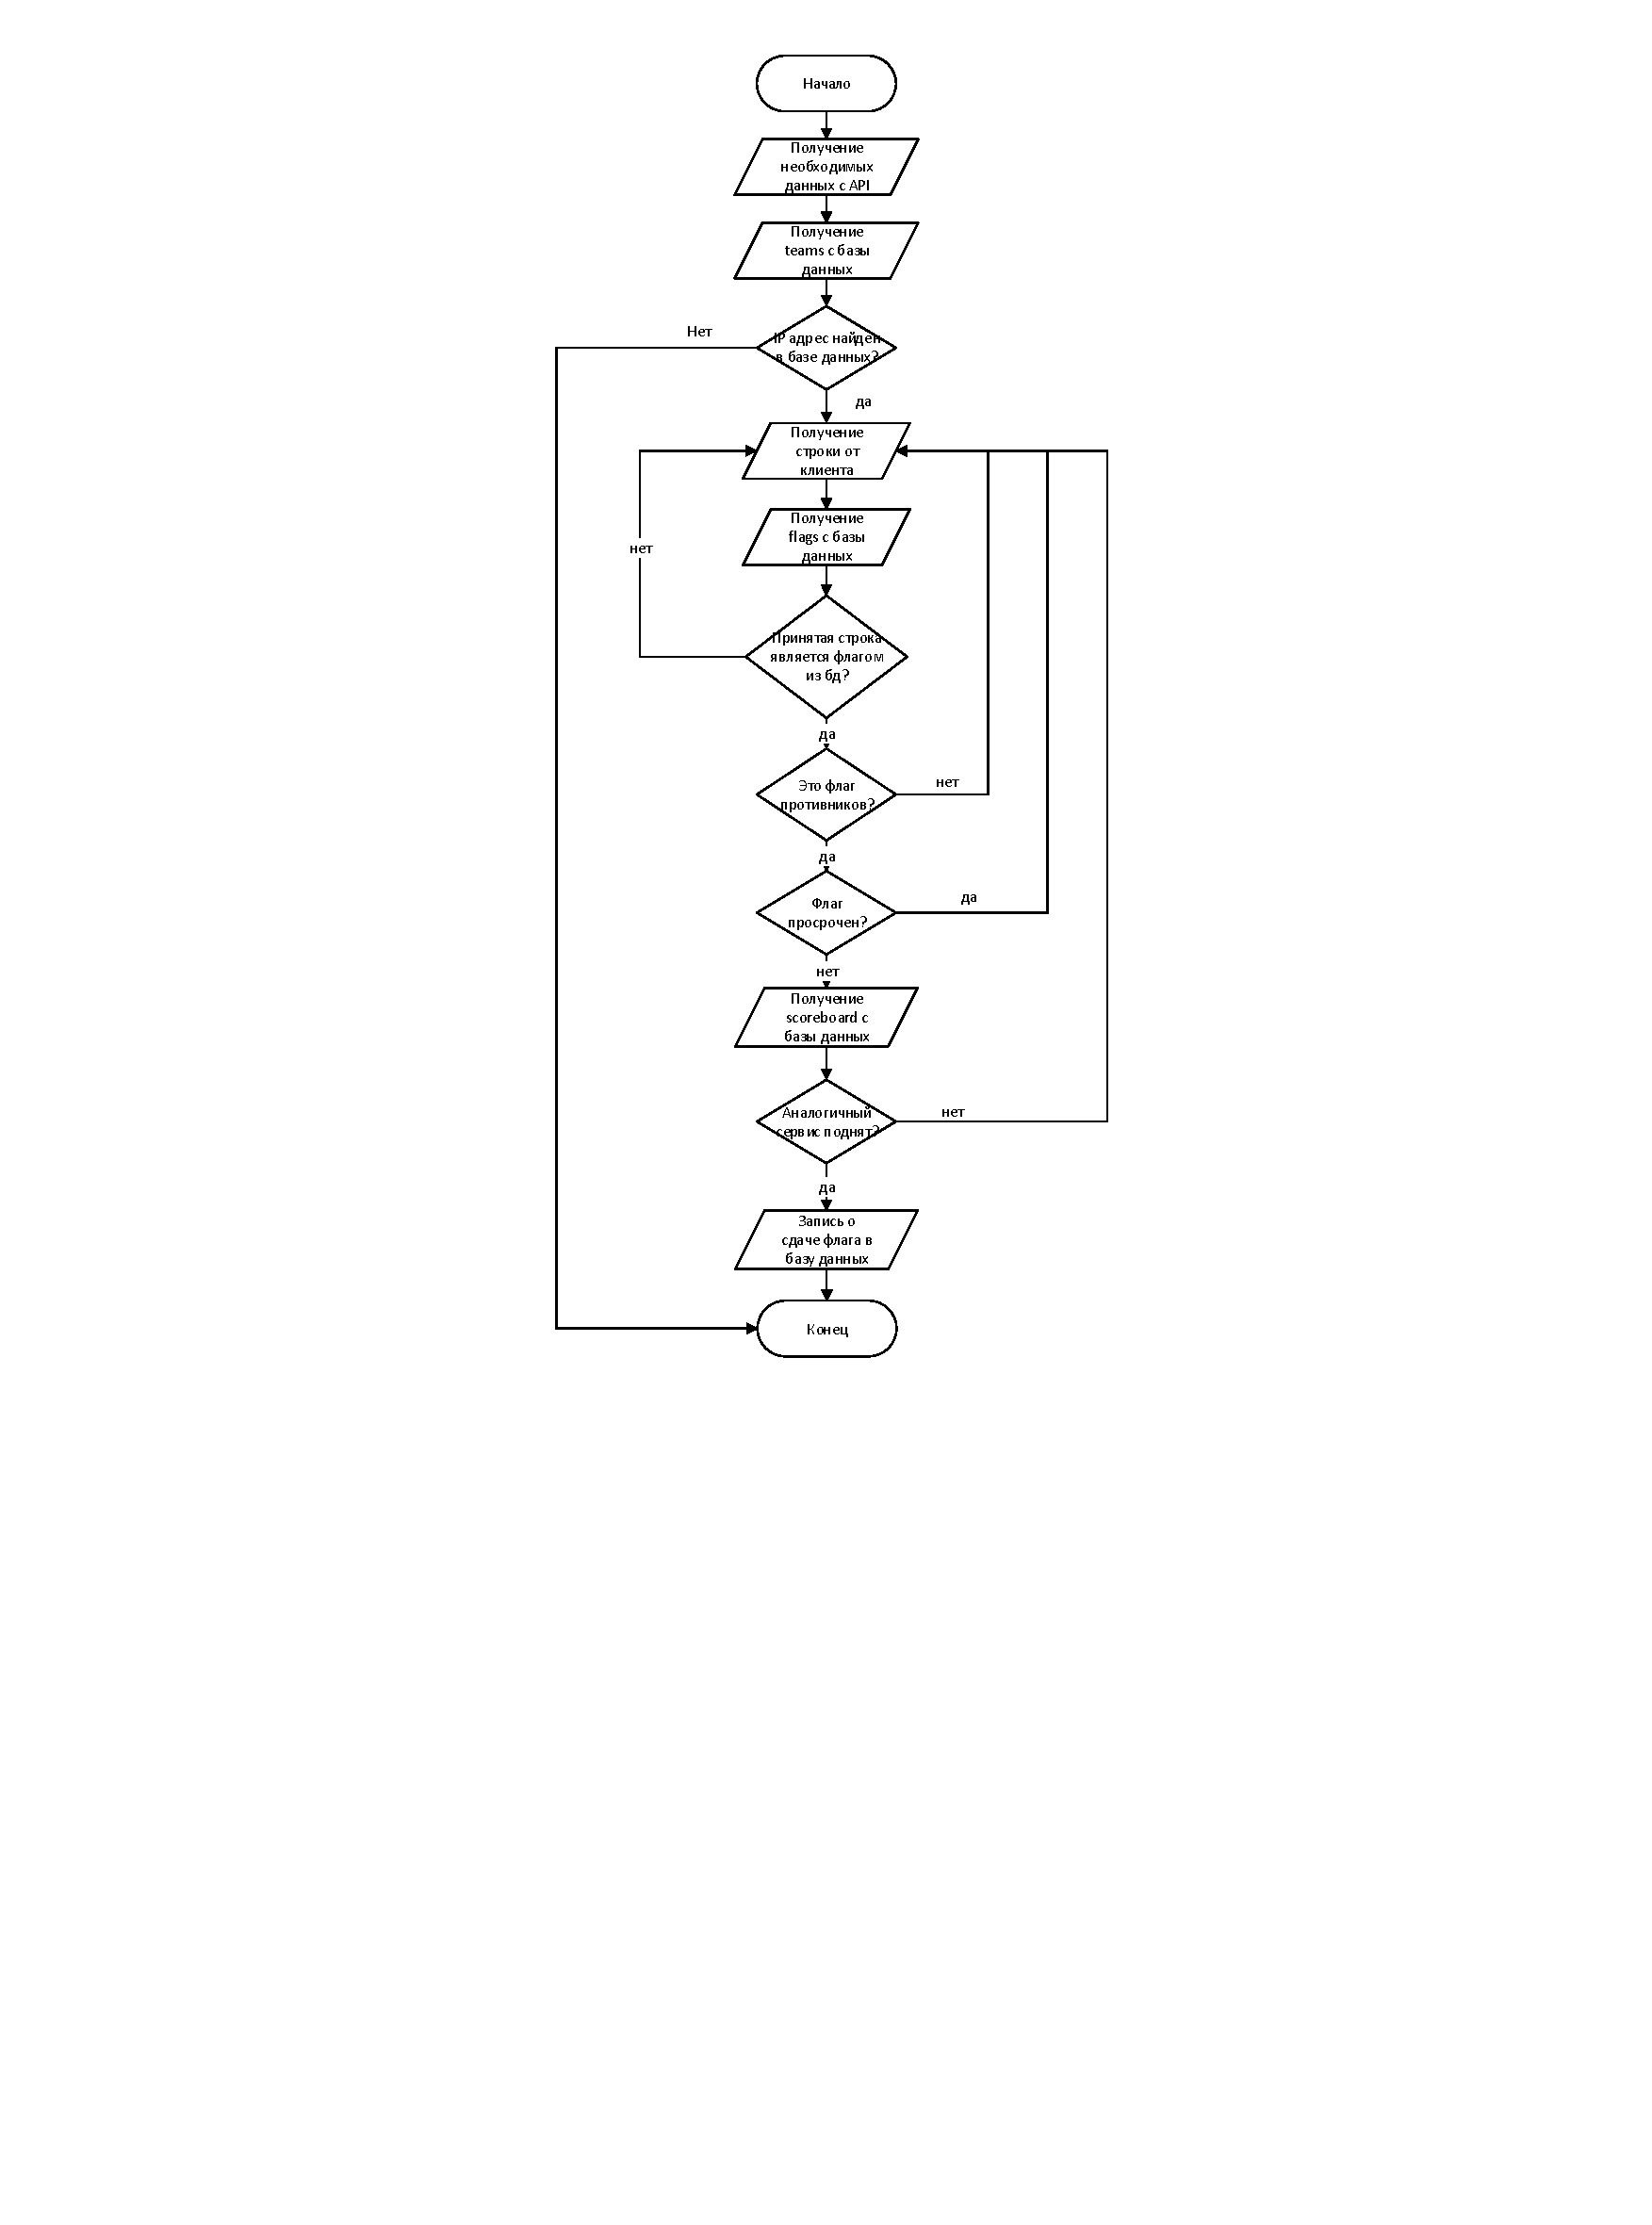
\includegraphics[trim=200 400 200 0, width=0.7\linewidth]{individual_reports/Algoritm.pdf}}
\caption{Алгоритм модуля flags.py}
\end{figure} 

\begin{figure}[h!]
\center{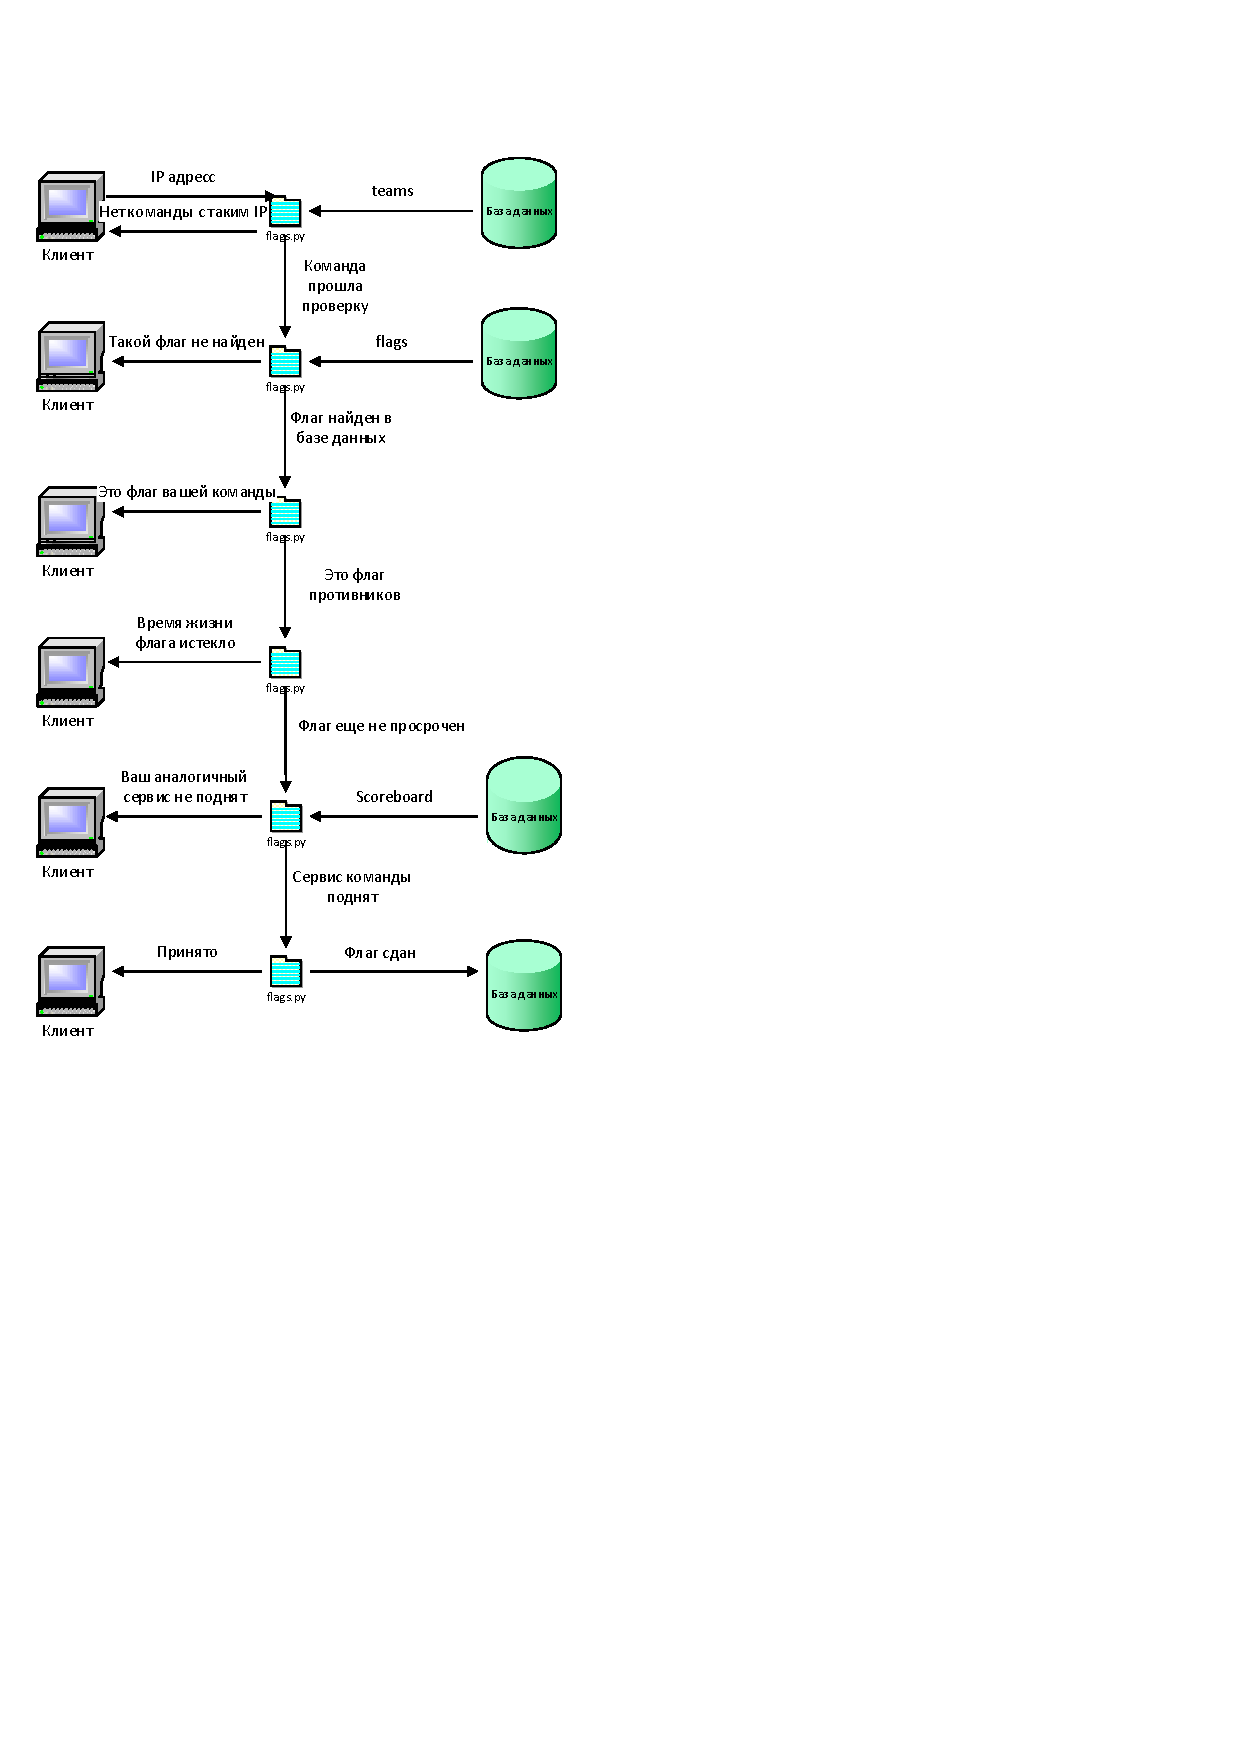
\includegraphics[trim=0 300 300 0, width=0.7\linewidth]{individual_reports/Naglyadno.pdf}}
\caption{Наглядная схема работы flags.py}
\end{figure} 

\clearpage


\subsection{Модуль: таблицы результатов} % - Отчёт scoreboard
В соревнованиях по информационной безопасности задача команд найти уязвимость и эксплуатировать её, добывая секретную информацию, в нашем случае флаги. Целью модуля является прием и проверка на валидность флагов.

\subsubsection{Принцип работы}

Программа реализована с использованием вебсокетов. На порту, полученном с API, программа сравнивает IP адрес клиента с данными в базе данных и при нахождении его, клиент определяется как одна из команд и может отправить серверу строку. Строка проверяется на длину символов. Так же флаг проверяется на наличие в базе данных, времени его жизни (флаги валидны определенное количество времени), принадлежность другой команде (свои флаги сдавать нельзя) и статус сервиса (аналогичный сервис сдающей команды должен быть поднят). 

Ниже представлен алгоритм и наглядная схема работы flags.py

\begin{figure}[h!]
\center{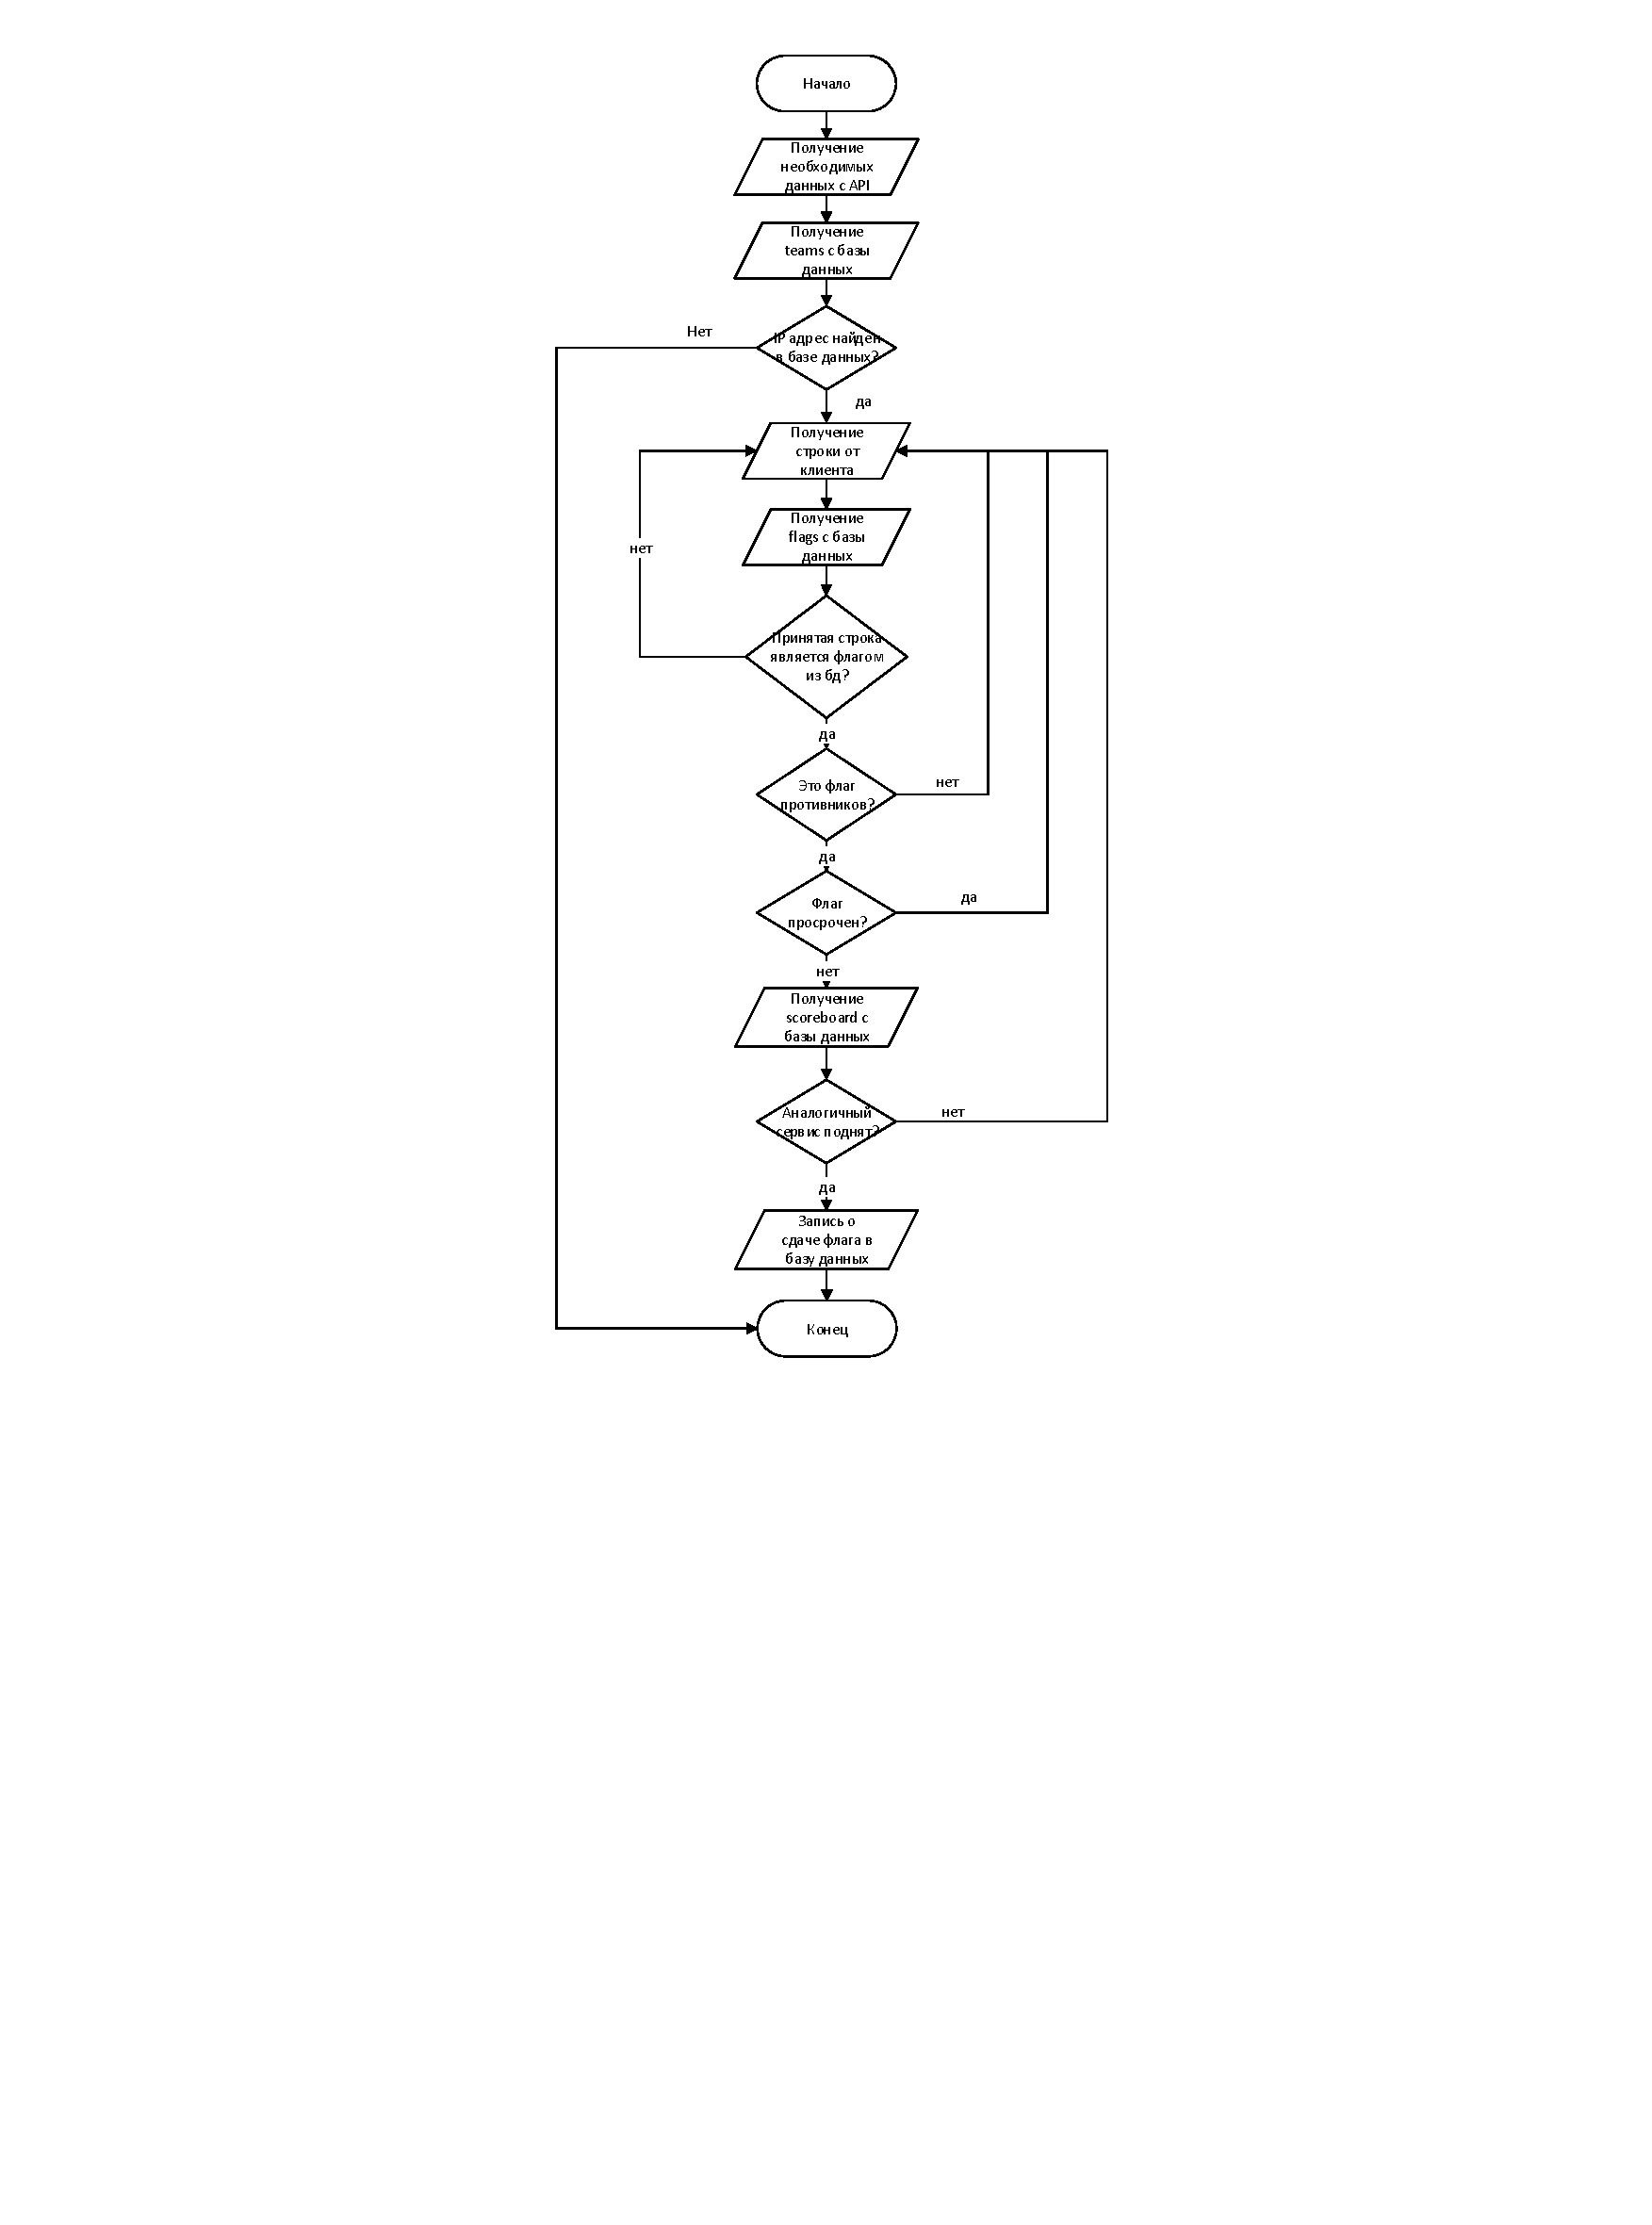
\includegraphics[trim=200 400 200 0, width=0.7\linewidth]{individual_reports/Algoritm.pdf}}
\caption{Алгоритм модуля flags.py}
\end{figure} 

\begin{figure}[h!]
\center{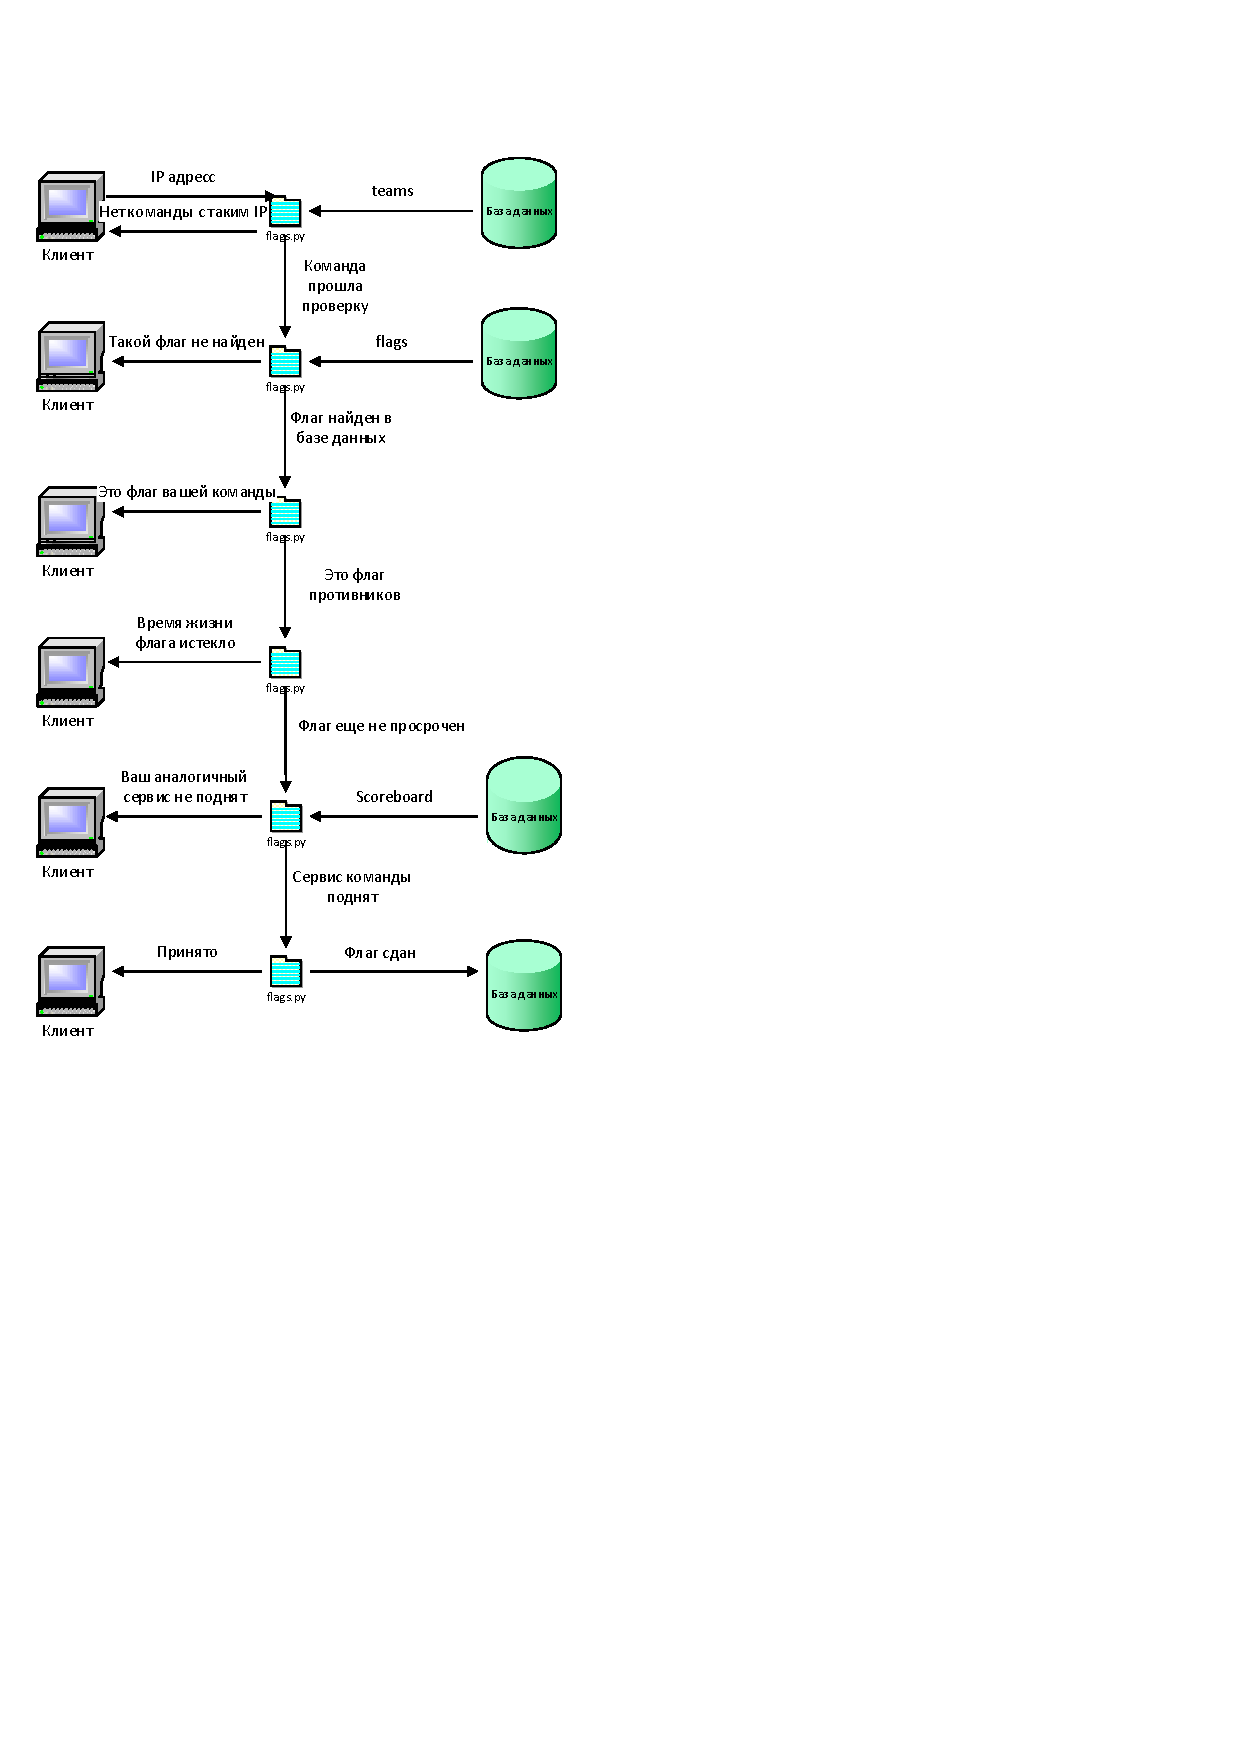
\includegraphics[trim=0 300 300 0, width=0.7\linewidth]{individual_reports/Naglyadno.pdf}}
\caption{Наглядная схема работы flags.py}
\end{figure} 

\clearpage


\subsection{Модуль: организации работы с сервисами} % - Отчёт round
Основное назначение платформы - общение с сервисами команд-участников посредством отправки и проверки специально сгенерированных флагов на сервере. Предназначение этого модуля - работа с интерфейсом сервисов (чекерами).

\subsubsection{Принцип работы}
Игра делится на раунды, каждый раунд, обычно, длится 1 минуту (настраивается при инициализации). Интерфейс для работы модуля с сервисом называется чекер. За этот период модуль опрашивает с помощью чекеров все сервисы команд-участников. Структура взаимодействия модуля с сервисами представлена на рисунке 5.4.

\begin{figure}[ht!]
\center{\includegraphics[width=1.0\linewidth]{images/module_round_structure.png}}
\caption{Иерархическая структура взаимодействия модуля с сервисами}
\end{figure}

Опрос происходит в три этапа:
\begin{enumerate} 
\item Проверка работоспособности сервиса команды-участника;
\item Отправление флага на сервис; 
\item Проверка того, что флаг сохранен.
\end{enumerate}

На каждом этапе модуль ожидает в ответ один из четырех чисел: 101, 102, 103, 104. Эти числа также называются статусом сервиса команды-участника. Алгоритм работы представлен на рисунке 5.5.

\begin{figure}[ht!]
\center{\includegraphics[width=0.5\linewidth]{images/module_round_schema.png}}
\caption{Схема создания потоков}
\end{figure}


Число 101 соответствует успешной работе сервиса команды-участника. Число 102 означает, что сервис команды работает, но на каком-то этапе отвечает некорректно. Число 103 означает, сервис команды отвечает, но не работает из-за какой-либо ошибки. Число 104 означает, что сервис команды не отвечает на запрос. 

Если на каком-то этапе чекер возвращает число отличное от 101, дальнейшее выполнение программы прекращается, а статус чекера записывается в базу данных.

На 1 этапе каждому чекеру посылается адрес сервера команды-участника. 
На 2 этапе каждому чекеру посылается адрес сервера, идентификатор флага и сам флаг. 
На 3 этапе каждому чекеру посылается адрес сервера, идентификатор флага и сам флаг.

Алгоритм работы представлен на рисунке 5.6.
\begin{figure}[ht!]
\center{\includegraphics[width=0.3\linewidth]{images/module_round_toservice.png}}
\caption{Блок-схема работы с каждым сервисом каждой команды-участника}
\end{figure}


Для увеличения производительности, каждый опрос сервисов команд-участников помещается в новый поток. Это позволяет работать в асинхронном режиме. Поэтому нестабильная работа сервиса команды-участника или ошибка в работе чекера не повлияет на опрос других сервисов. Также каждому потоку задается ограничение по времени работы. Это позволяет своевременно завершать процессы, тем самым уменьшается нагрузка на процессор и на потребление памяти.



\clearpage

\newpage
\subsection{Сбор информации из браузера Google Chrome} % - Отчёт Влада
Целью работы в текущем семестре являлось исследование журнальных файлов и доработка программного модуля для сбора пользовательских данных приложения Google Chrome и представления их в формате XML.

В ходе изучения работы данного браузера было установлено, что приложение Google Chrome хранит пользовательские данные локально. Адреса директорий, используемых по умолчанию для этих целей Google Chrome можно увидеть в таблице~\ref{tab:tab_1}, пользовательские данные --- в таблице~\ref{tab:tab_2}.

\begin{table}[ht]
\caption{Директории хранения журнальных файлов Chrome}
\label{tab:tab_1}
\begin{center}
\begin{tabularx}{\linewidth}{|l|X|}
\hline
Операционная система & Директория \\
\hline
Linux (Debian) & /home/имя пользователя/.config/google-chrome/Default/ \\
\hline
Win7 & C:\textbackslash Users\textbackslash имя пользователя \textbackslash AppData\textbackslash Local\textbackslash Google \\
 & \textbackslash Chrome\textbackslash User Data\textbackslash Default\textbackslash \\
\hline
Win8 & C:\textbackslash Users\textbackslash имя пользователя \textbackslash AppData\textbackslash Local\textbackslash Google \\
 & \textbackslash Chrome\textbackslash User Data\textbackslash Default\textbackslash \\
\hline
\end{tabularx}
\end{center}
\end{table}

\begin{table}[ht]
\caption{Пользовательские данные}
\label{tab:tab_2}
\begin{center}
\begin{tabularx}{\linewidth}{|l|X|}
\hline
Файл & Содержание \\
\hline
Bookmarks & Закладки \\
\hline
History & История посещений, история запросов, история загруженных файлов \\
\hline
Preferences & Настройки (директория загрузки файлов, версия программы, логин аккаунта Google) \\
\hline
Login Data & Сохраненные логины и пароли \\
\hline
Extensions (папка) & Расширения \\
\hline
\end{tabularx}
\end{center}
\end{table}

\subsubsection{База данных Login Data Chrome}

Login Data --- это реляционная база данных, основанная на СУБД SQLite.
Необходимо рассмотреть данную БД, которая содержит 2 таблицы:

\begin{enumerate}
  \item logins;
  \item meta.
\end{enumerate}

Интерес представляет только таблица logins. Она содержит следующие поля:

\begin{enumerate}
  \item origin\_url --- адрес ресурса;
  \item username\_value --- логин для доступа;
  \item password\_value --- пароль, представленный в виде BLOB массива двоичных данных (Binary Large OBject);
  \item date\_created --- дата сохранения, представленная в следующем виде (пример): 13072972925957814. Это число есть количество секунд, прошедшее с 00:00:00 UTC 1 января, 1601 года (рис.~\ref{ship_1:ship_1}).
\end{enumerate}

\begin{figure}[h!]
\center{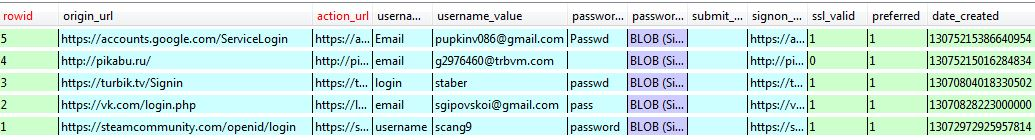
\includegraphics[width=0.9\linewidth]{ship_1}}
\caption{Структура таблицы login}
\label{ship_1:ship_1}
\end{figure} 

Запрос для импорта данных выглядит следующим образом:

\begin{verbatim}
SELECT logins.origin_url,
       logins.username_value,
       datetime(logins.date_created/1000000 + 
       (strftime('%s','1601-01-01')),'unixepoch')
FROM logins;
\end{verbatim}

Результат выполнения запроса можно увидеть на рисунке~\ref{ship_2:ship_2}, блок-схему алгоритма выборки данных из БД Login Data --- на рисунке~\ref{ship_3:ship_3}. Результат выполнения программы в формате XML --- рисунок~\ref{ship_4:ship_4}.

Значение поля id --- уникальный идентификатор для последующего импорта в solr БД и работы с ним.

\begin{figure}[h!]
\center{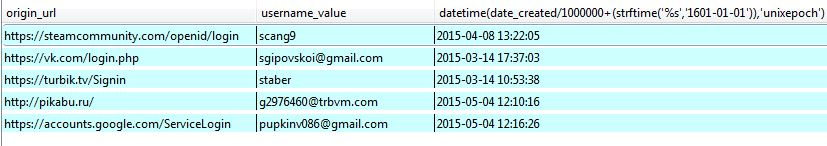
\includegraphics[width=0.9\linewidth]{ship_2}}
\caption{Результат выполнения запроса}
\label{ship_2:ship_2}
\end{figure}

\begin{figure}[h!]
\center{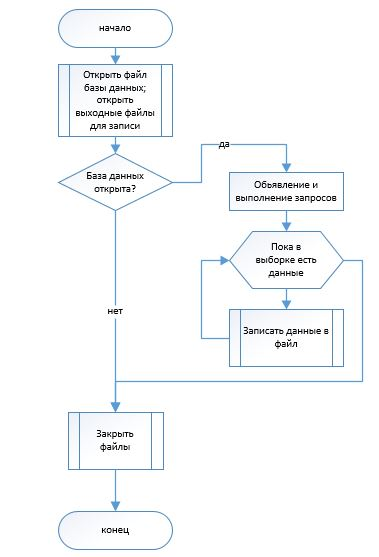
\includegraphics[width=0.5\linewidth]{ship_3}}
\caption{Блок-схема алгоритма выборки данных из БД Login Data}
\label{ship_3:ship_3}
\end{figure} 

\begin{figure}[h!]
\center{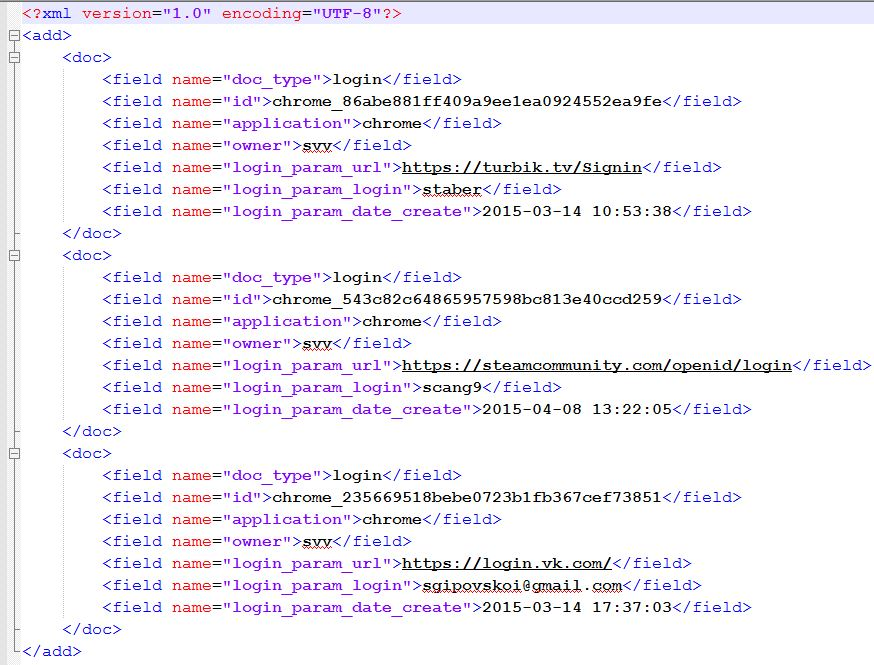
\includegraphics[width=0.7\linewidth]{ship_4}}
\caption{Файл login.XML}
\label{ship_4:ship_4}
\end{figure} 

\clearpage
\subsubsection{Расширения браузера Chrome (Extensions)}

В папке Extensions (рис.~\ref{ship_5:ship_5}) находятся данные об установленных в брузере расширениях. Для каждого расширения имеется своя папка, в которой находится различная информация. Также для каждого Extension имеется файл manifest (рис.~\ref{ship_6:ship_6}) с расширением JSON. JSON (JavaScript Object Notation) --- текстовый формат обмена данными, основанный на JavaScript. Из данного файла необходима только информация об имени и версии расширения.

Блок-схему алгоритма импорта данных о расширениях можно увидеть на рисунке~\ref{ship_7:ship_7}. 

\begin{figure}[h!]
\center{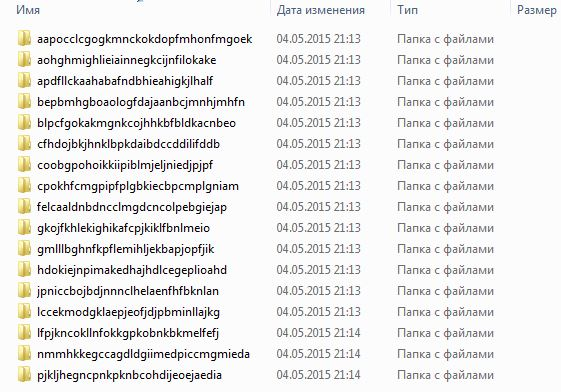
\includegraphics[width=0.6\linewidth]{ship_5}}
\caption{Папка Extensions}
\label{ship_5:ship_5}
\end{figure}

\begin{figure}[h!]
\center{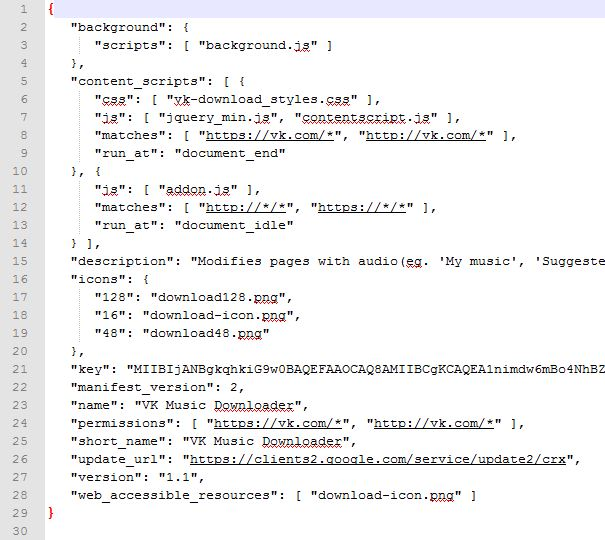
\includegraphics[width=0.6\linewidth]{ship_6}}
\caption{Файл manifest.json}
\label{ship_6:ship_6}
\end{figure}

\begin{figure}[h!]
\center{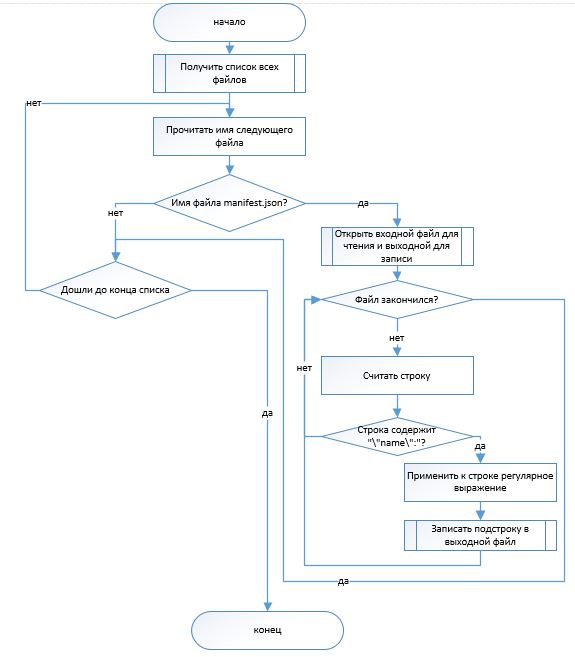
\includegraphics[width=0.8\linewidth]{ship_7}}
\caption{Блок-схема алгоритма импорта данных о расширениях}
\label{ship_7:ship_7}
\end{figure}

\clearpage
Извлечение подстроки из строки осуществляется с помощью регулярного выражения \textbackslash"(.*)\textbackslash".*\textbackslash"(.*)\textbackslash". Например, есть строка <<name>>: <<VK Music Downloader>>. Данное регулярное выражение возвращает 2 подстроки --- <<name>> и <<VK Music Downloader>>, что и требовалось в ходе работы.

Результат был записан в файл extensions.XML (рис.~\ref{ship_8:ship_8}).

\begin{figure}[h!]
\center{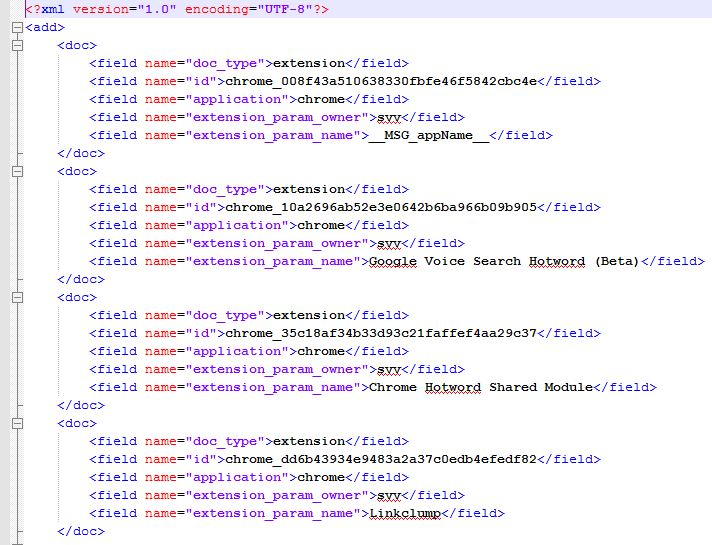
\includegraphics[width=0.7\linewidth]{ship_8}}
\caption{Файл extensions.XML}
\label{ship_8:ship_8}
\end{figure}

\subsubsection{Изменения, добавленные в программный модуль в течение текущего семестра}

В файл bookmarks.XML добавлены 2 поля (рис.~\ref{ship_9:ship_9}):

\begin{enumerate}
  \item дата добавления закладки;
  \item владелец файла.
\end{enumerate}

\begin{figure}[h!]
\center{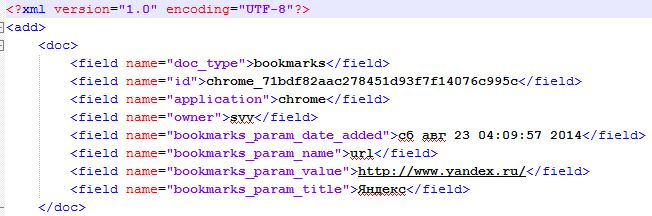
\includegraphics[width=0.7\linewidth]{ship_9}}
\caption{Файл bookmarks.XML}
\label{ship_9:ship_9}
\end{figure}

В файл history.XML (рис.~\ref{ship_10:ship_10}) добавлено поле-дата последнего посещения ресурса.

\begin{figure}[h!]
\center{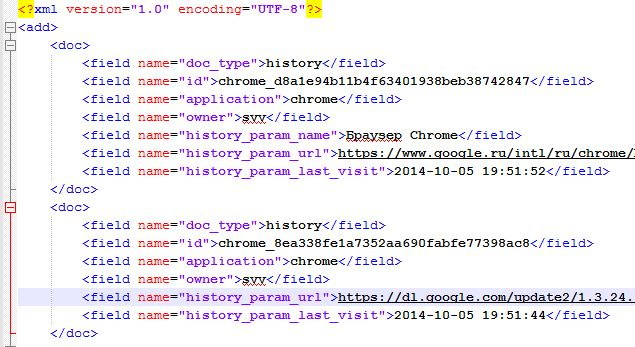
\includegraphics[width=0.8\linewidth]{ship_10}}
\caption{Файл history.XML}
\label{ship_10:ship_10}
\end{figure}

Также было реализовано преобразование данных времени начала и конца загрузки, а также о количестве занимаемого места к читаемому виду (рис.~\ref{ship_11:ship_11}).

\begin{figure}[h!]
\center{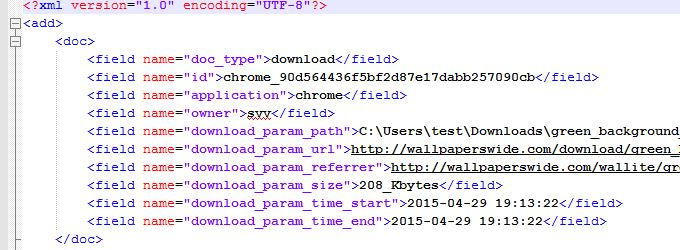
\includegraphics[width=0.8\linewidth]{ship_11}}
\caption{Файл downloads.XML}
\label{ship_11:ship_11}
\end{figure}

\clearpage
Помимо этого реализованы следующие задачи:

\begin{enumerate}
  \item присоединение модуля к общей системе coex;
  \item рекурсивный обход файловой системы для нахождения входных файлов;
  \item различие выходных данных при обработке входных от нескольких пользователей путём добавления в конец имени файла даты и количества наносекунд, прошедших с начала работы функции.
\end{enumerate}

На данный момент реализован импорт следующих данных:

\begin{enumerate}
  \item история посещений;
  \item история загруженных файлов;
  \item история поисковых запросов;
  \item список установленных расширений;
  \item информация о версии программы, подключённом аккаунте google;
  \item сохраненные данные для доступа к ресурсам(только логин).
\end{enumerate}

Список всех выходных XML-файлов приведен на рисунке~\ref{ship_12:ship_12}.

\begin{figure}[h!]
\center{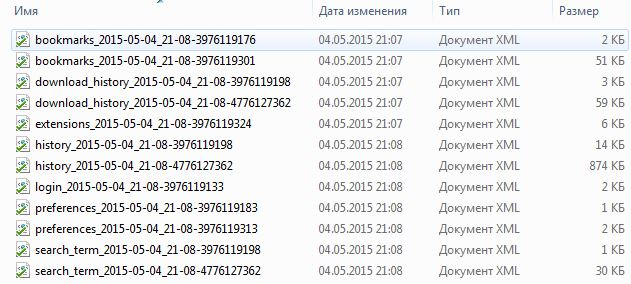
\includegraphics[width=0.7\linewidth]{ship_12}}
\caption{Файл downloads.XML}
\label{ship_12:ship_12}
\end{figure}


\newpage
\subsection{Модуль: прием и проверка принятых флагов} % - Отчёт flags
В соревнованиях по информационной безопасности задача команд найти уязвимость и эксплуатировать её, добывая секретную информацию, в нашем случае флаги. Целью модуля является прием и проверка на валидность флагов.

\subsubsection{Принцип работы}

Программа реализована с использованием вебсокетов. На порту, полученном с API, программа сравнивает IP адрес клиента с данными в базе данных и при нахождении его, клиент определяется как одна из команд и может отправить серверу строку. Строка проверяется на длину символов. Так же флаг проверяется на наличие в базе данных, времени его жизни (флаги валидны определенное количество времени), принадлежность другой команде (свои флаги сдавать нельзя) и статус сервиса (аналогичный сервис сдающей команды должен быть поднят). 

Ниже представлен алгоритм и наглядная схема работы flags.py

\begin{figure}[h!]
\center{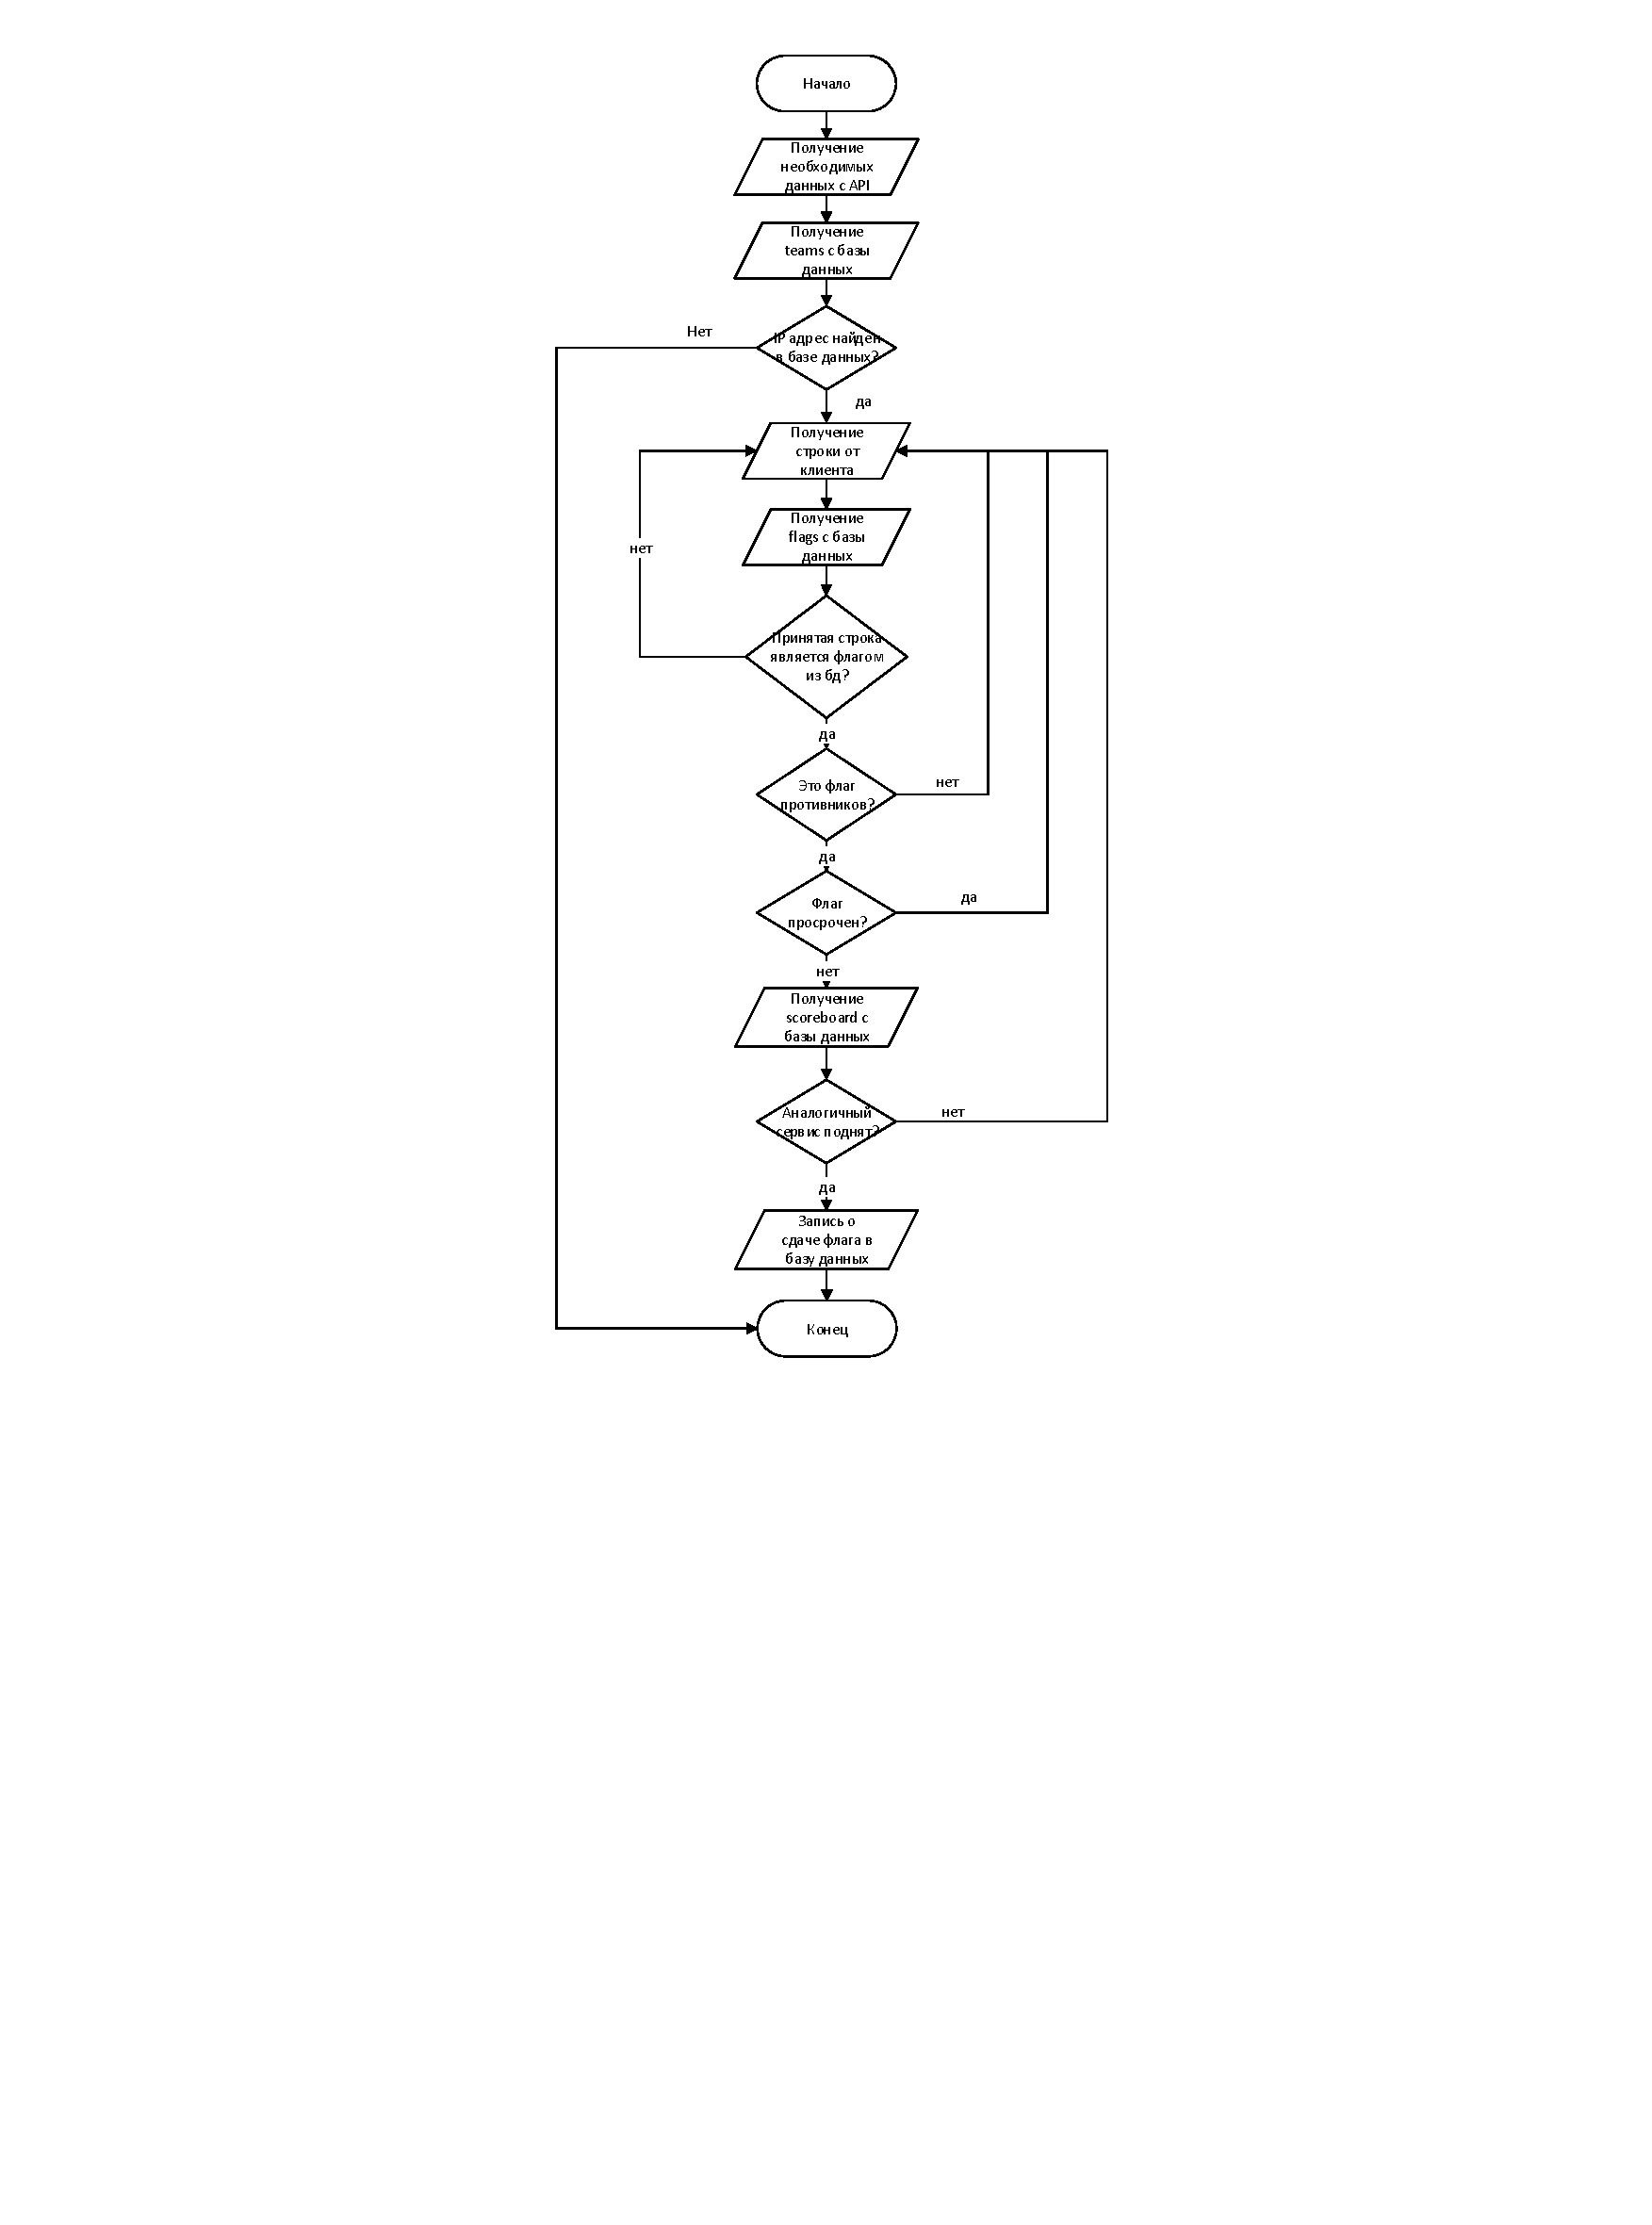
\includegraphics[trim=200 400 200 0, width=0.7\linewidth]{individual_reports/Algoritm.pdf}}
\caption{Алгоритм модуля flags.py}
\end{figure} 

\begin{figure}[h!]
\center{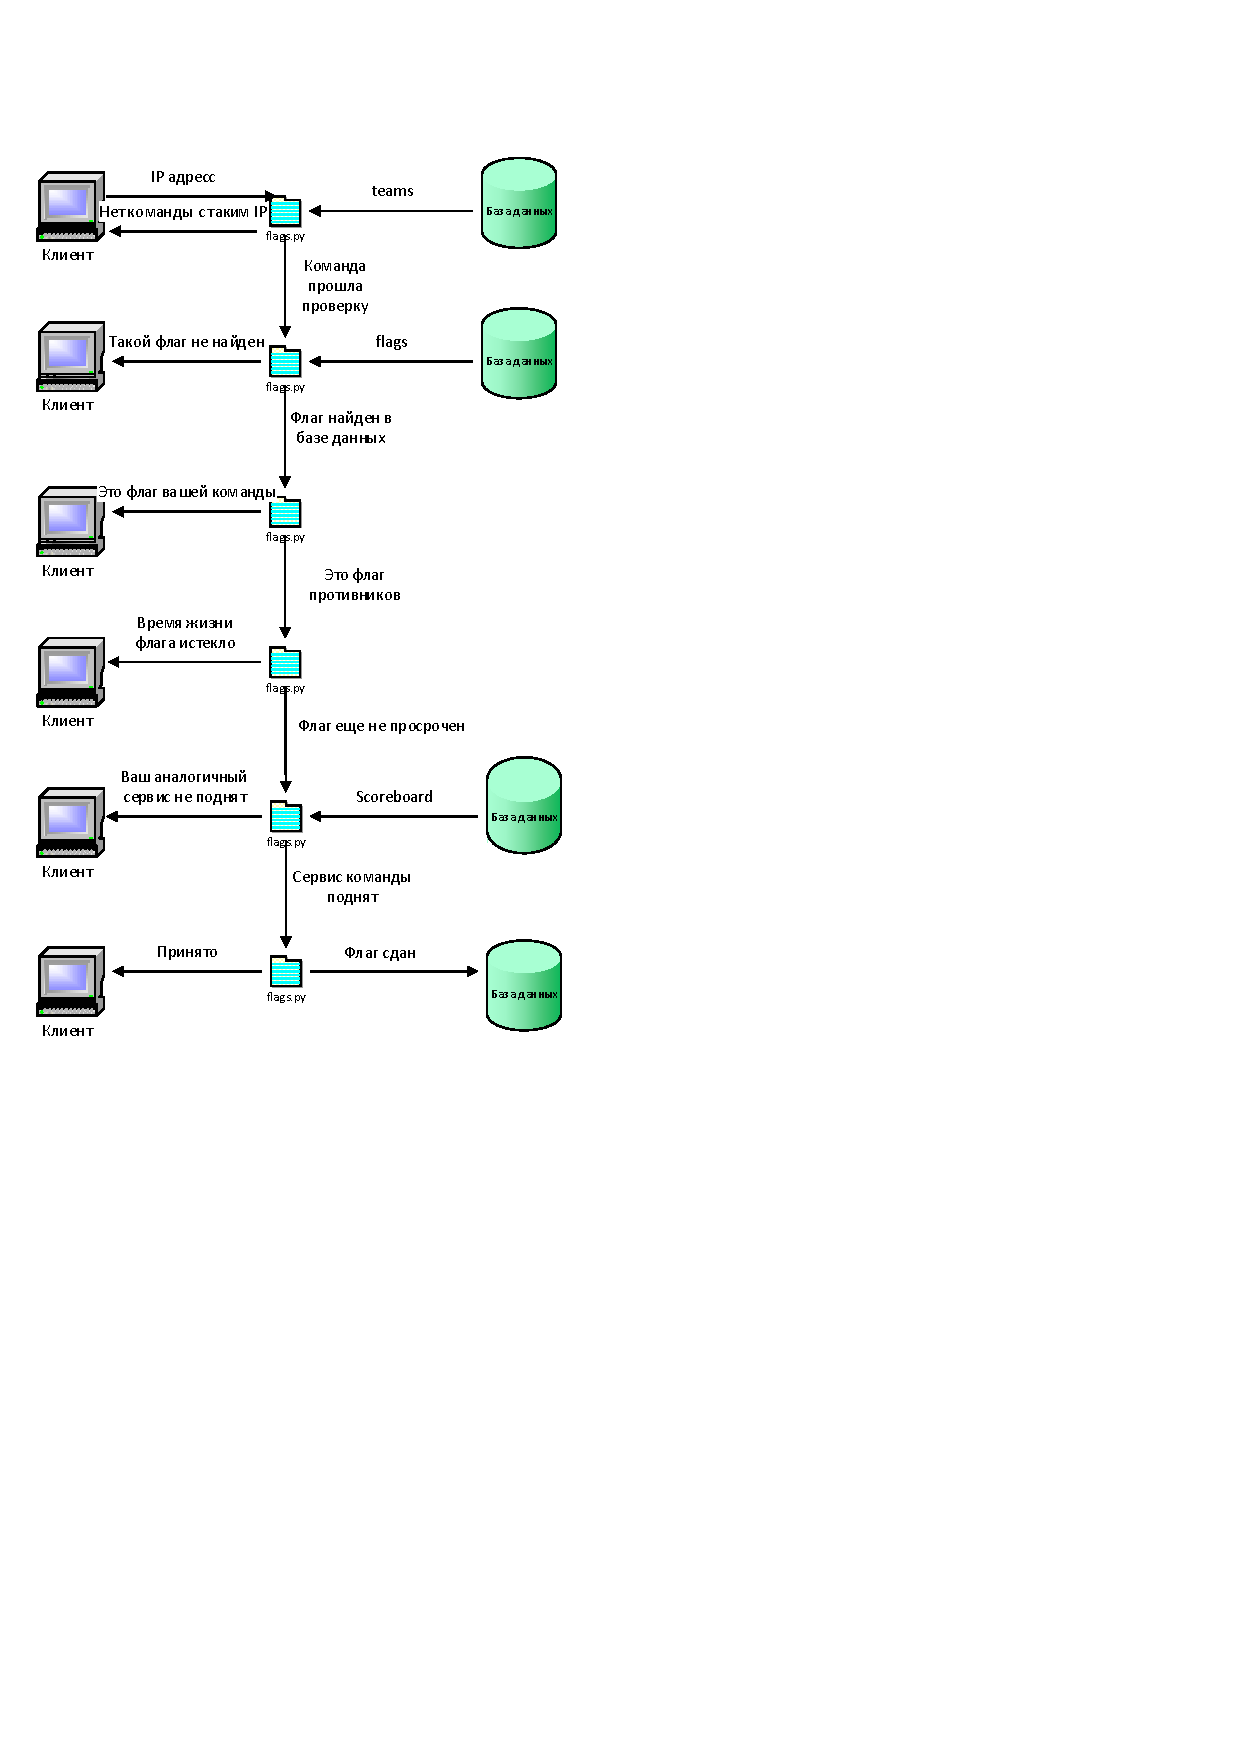
\includegraphics[trim=0 300 300 0, width=0.7\linewidth]{individual_reports/Naglyadno.pdf}}
\caption{Наглядная схема работы flags.py}
\end{figure} 

\clearpage


\newpage
\subsection{Cбор информации из почтового клиента MS Outlook} % - Отчет Андрея
В ходе проведения компьютерной экспертизы может возникнуть необходимость 
проанализировать электронные письма злоумышлиника. Подобную информацию можно 
получить из файлов, сохраняемых программой OutLook на ПК пользователя. Для 
осуществления данной задачи был разработан программный модуль Outlook.

Почтовая программа (почтовый клиент, клиент электронной почты, мейлер, мейл-клиент) --- 
это ПО, которое инсталлируется на компьютер пользователя и предназначено для 
написания, получения, хранения, отправки электронной почты одного или нескольких 
пользователей (например, когда имеется несколько учетных записей на компьютере), или 
нескольких учетных записей пользователя.

Сообщения, синхронизированные с Outlook, имеют самой программе следующий вид (рис~\ref{ser_1:ser_1}). Задача 
модуля состоит из поиска данных, отображаемых в программе Outlook в бинарном файле <<.dbx>> (рис~\ref{ser_2:ser_2}). В результате работы модуля получаем списки всех тем, дат и тд. сообщения (рис~\ref{ser_3:ser_3}).

\begin{figure}[h!]
\center{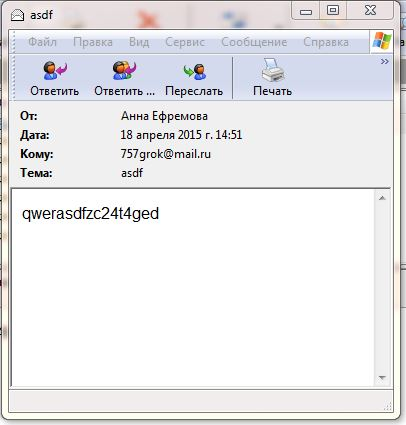
\includegraphics[width=0.6\linewidth]{ser_1}}
\caption{Сообщения, синхронизированные с Outlook}
\label{ser_1:ser_1}
\end{figure} 

\begin{figure}[h!]
\center{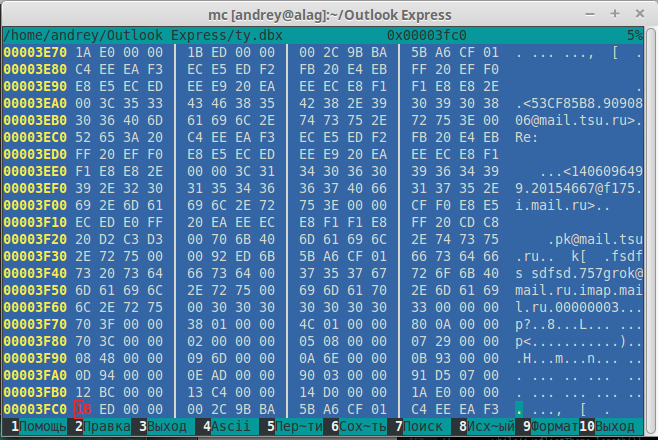
\includegraphics[width=0.8\linewidth]{ser_2}}
\caption{Содержание бинарного файла формата <<.dbx>>}
\label{ser_2:ser_2}
\end{figure} 

\begin{figure}[h!]
\center{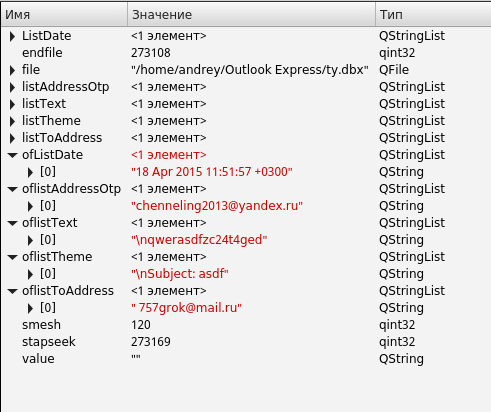
\includegraphics[width=0.8\linewidth]{ser_3}}
\caption{Результат работы модуля}
\label{ser_3:ser_3}
\end{figure} 

\clearpage
\subsubsection{Реализация программного модуля для почтового клиента MS Outlook}

Реализация данного программного модуля включала в себя следующие шаги:

\begin{enumerate}
  \item изучение бинарного формата данных <<.dbx>>;
  \item изучение регулярных выражений и библиотек для работы с ними в Qt C++;
  \item разработка поиска файлов формата <<.dbx>> на носителе, на котором установлен Outlook;
  \item разработка программы для считывания не всего файла, а только его части, чтобы тем самым 
  уменьшить нагрузку на оперативную память;
  \item разработка регулярных выражений для поиска адресата, отправителя, темы, даты и 
  текста сообщения и создание парсера для части информации, извлекаемой из файла;
  \item изучение особенностей работы с XML-форматом (языком разметки) и разработка класса для 
  записи данных, полученных из парсера, в XML;
  \item изучение системы распределенного контроля версий Git и ее основных возможностей;
  \item изучение различных файловых форматов, таких как PST, PAB, MSG, RTF, HTML.  
\end{enumerate}

Трудности, возникшие при написании модуля:

\begin{enumerate}
  \item В начале написания модуля  возникла явная проблема переполнения оперативной 
  памяти из-за добавления всего файла целиком в поток главной программы. 
  Появилась потребность в написании программы, которая делила бы файл на части, 
  запоминала место конца предыдущей части программы и начинала отделять часть 
  такой же длины. Кроме того, данная программа должна была считывать часть файла из любого его места, 
  которую укажут в параметрах, а также преобразовывать последовательность бит в строку юникода. 
  После чего была разработана и написана программа, реализующая данную потребность.
  \item Далее стала необходимой разработка парсера (некоего фильтра данных), который бы находил и 
  забирал из выбранной части файла нужные нам последовательности бит. Были изучены основы регулярных 
  выражений, а также синтаксис составления шаблонов для класса QTRegex, реализующего работу с  
  регулярными выражениями в QT C++, включая сам класс QTRegex. Блок-схема данного парсера представлена 
  на рисунке~\ref{ser_4:ser_4}.
  \item Далее необходимо было разработать алгоритм занесения полученных данных в какой-либо 
  файл для их хранения. В связи с тем, что проект <<coex>> использует для вывода данных 
  файлы формата XML, был изучен данный формат, а также классы для работы с ним в QT C++. 
  После чего был написан класс <<WriteAddress>>, осуществляющий запись данных из парсера в XML. 
\end{enumerate}

Блок-схема исходного модуля после всех преобразований и дополнений приняла следующий вид
(рис.~\ref{ser_5:ser_5}).

\begin{figure}[h!]
\center{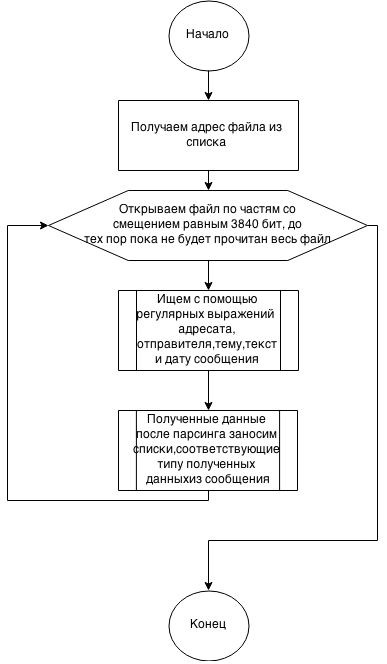
\includegraphics[width=0.6\linewidth]{ser_4}}
\caption{Блок-схема парсера для работы с битовыми строками}
\label{ser_4:ser_4}
\end{figure} 

\begin{figure}[h!]
\center{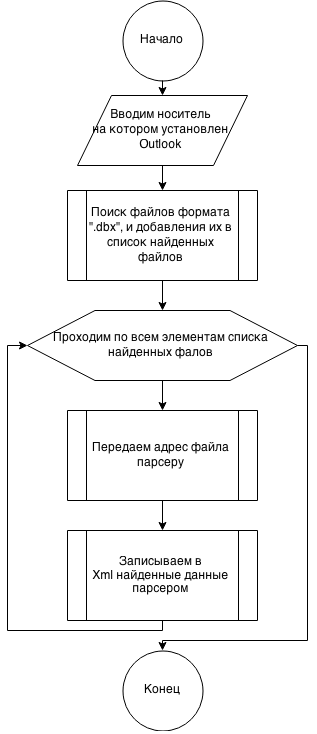
\includegraphics[width=0.5\linewidth]{ser_5}}
\caption{Блок-схема исходного модуля Outlook}
\label{ser_5:ser_5}
\end{figure} 

\subsubsection{Задачи на следующий семестр}

В следующем семестре планируется переделать поиск фалов не только в стандартном 
расположении (месте установки) Outlook, но и в других директориях, за непродолжительное 
время. Также планируется увеличить скорость работы модуля путем распараллеливания  потоков.

\clearpage


\newpage
\subsection{Cбор информации из почтового клиента Mozilla Thunderbird}  % - Отчет Юры
Целью данной работы стало исследование почтового клиента Mozilla Thunderbird, написание программного модуля для сбора сообщений и представления их в формате XML.

\subsubsection{Реализация программного модуля}

В ходе изучения приложения было выяснено расположение файлов, хранящих почтовые сообщения. Эти данные представлены в таблице~\ref{tab:data}, где:

\begin{itemize}
  \item profile\_name --- может быть любым и генерируется самой программой (например, g5bq66yo.default);
  \item server\_name --- название сервера входящей почты (например, imap.yandex.com).
\end{itemize}

\begin{table}[ht]
\caption{Местоположение и название файлов}
\label{tab:data}
\begin{center}
\begin{tabularx}{\linewidth}{|X|X|X|X|}
\hline
Протокол & Путь & Файл с входящими сообщениями & Файл с исходящими сообщениями \\
\hline
imap & C:\textbackslash Users\textbackslash User\textbackslash AppData   & INBOX & \textampersand BB4EQgQ,BEAEMAQ\\
     & \textbackslash Roaming\textbackslash Thunderbird                  &       & yBDsENQQ9BD0ES \\
     & \textbackslash Profiles\textbackslash profile\_name  &   & wQ1- \\
     & \textbackslash ImapMail\textbackslash server\_name   &   &      \\
\hline
pop3 & C:\textbackslash Users\textbackslash User\textbackslash AppData & Inbox & Sent \\
     & \textbackslash Roaming\textbackslash Thunderbird                &       &      \\
     & \textbackslash Profiles\textbackslash profile\_name             &       &      \\
     & \textbackslash Mail\textbackslash server\_name                  &       &      \\
\hline
\end{tabularx}
\end{center}
\end{table}

Для каждого почтового аккаунта, который подключен в Thunderbird, создается своя папка <<server\_name>>. Данные указаны для windows 7, 8, 8.1.

Проводник Windows не может определить расширение файлов, но при открытии любым текстовым редактором можно понять, что файлы имеют формат mbox. Mbox представляет собой текстовый файл, в котором хранятся все сообщения почтового ящика. Начало почтового сообщения определяется строкой из 5 символов: словом <<From>> с последующим пробелом.

Пример сообщения:

\begin{verbatim}
  From 
  Message-ID: <55600F73.6020804@yandex.ru>
  Date: Sat, 23 May 2015 11:26:11 +0600
  From: fgfgsr <art0rias@yandex.ru>
  User-Agent: Mozilla/5.0 (Windows NT 6.1; WOW64; rv:31.0) 
              Gecko/20100101 Thunderbird/31.7.0
  MIME-Version: 1.0
  To: yuriy94@hotmail.com
  Content-Type: text/plain; charset=utf-8; format=flowed
  Content-Transfer-Encoding: 7bit

  Little girl, little girl, Where have you been?
\end{verbatim}

В блоке с сообщением хранятся данные о дате, отправителе, получателе, версии почтового клиента, является ли письмо ответом на другое, а также заголовок и текст письма.

\subsubsection{Алгоритм работы модуля}

После открытия файл mbox разделяется на отдельные сообщения с помощью регулярного выражения <<(From \textbackslash \textbackslash r\textbackslash \textbackslash n)|(From \textbackslash \textbackslash n\textbackslash \textbackslash r)|From \textbackslash \textbackslash r|From \textbackslash \textbackslash n>>. Затем к каждому сообщению применяются регулярные выражения:

\begin{itemize}
  \item <<\textbackslash \textbackslash nDate: ([\textasciicircum \textbackslash \textbackslash n]*)\textbackslash \textbackslash n>> --- время отправки/приема сообщения;
  
  \item <<\textbackslash \textbackslash nFrom: .*([a-z][\textbackslash \textbackslash w\textbackslash \textbackslash .]*\textbackslash \textbackslash w@\textbackslash \textbackslash w[\textbackslash \textbackslash w\textbackslash \textbackslash .]*\textbackslash \textbackslash .\textbackslash \textbackslash w*).*\textbackslash \textbackslash nUser-Agent:>> --- кто отправил сообщения;
  
  \item <<\textbackslash \textbackslash nTo: .*([a-z][\textbackslash \textbackslash w\textbackslash \textbackslash .]*\textbackslash \textbackslash w@\textbackslash \textbackslash w[\textbackslash \textbackslash w\textbackslash \textbackslash .]*\textbackslash \textbackslash .\textbackslash \textbackslash w*).*\textbackslash \textbackslash nSubject:>> --- кто получил сообщение;
  
  \item <<\textbackslash \textbackslash nContent-Transfer-Encoding: 8bit\textbackslash \textbackslash s*(\textbackslash \textbackslash S.*\textbackslash \textbackslash S)\textbackslash \textbackslash s*[0-3]\textbackslash \textbackslash d\textbackslash \textbackslash .[01]\textbackslash \textbackslash d\textbackslash \textbackslash .\textbackslash \textbackslash d{4} [0-2]\textbackslash \textbackslash d:[0-5]\textbackslash \textbackslash d, [\textasciicircum \textbackslash \textbackslash n]*\textbackslash \textbackslash n>> --- текст сообщения.
\end{itemize}

Блок-схема алгоритма представлена на рисунке~\ref{teresh_1:teresh_1}.

\begin{figure}[h!]
\center{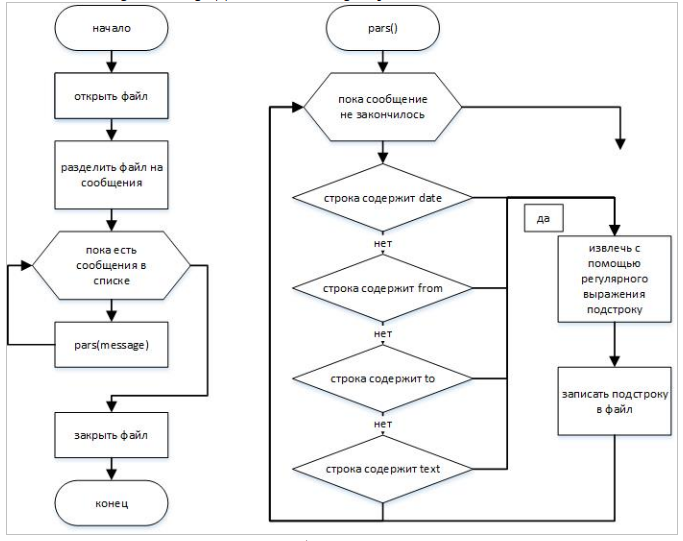
\includegraphics[width=0.9\linewidth]{teresh_1}}
\caption{Блок-схема алгоритма}
\label{teresh_1:teresh_1}
\end{figure}

\clearpage

\subsubsection{Структура XML-файла}

Документы XML имеют иерархическую структуру и начинаются с элемента <add> --- это начальный элемент документа (корень). Далее будут записаны n дочерних элементов <file>, где n --- количество файлов mbox. В каждый элемент <file> будут записаны m дочерних элементов <message>, где m --- количество сообщений в одном файле, в теле которых будет записано нужное нам количество полей для записи информации. В последнюю очередь записывается конечный элемент </add>.

Пример файла message\_report.xml приведен на рисунке~\ref{teresh_2:teresh_2}.

Значения полей date, from, to, text содержат время и дату, отправителя, получателя, текст сообщения соответственно. Поле name содержит полный путь к mbox файлу.

\begin{figure}[h!]
\center{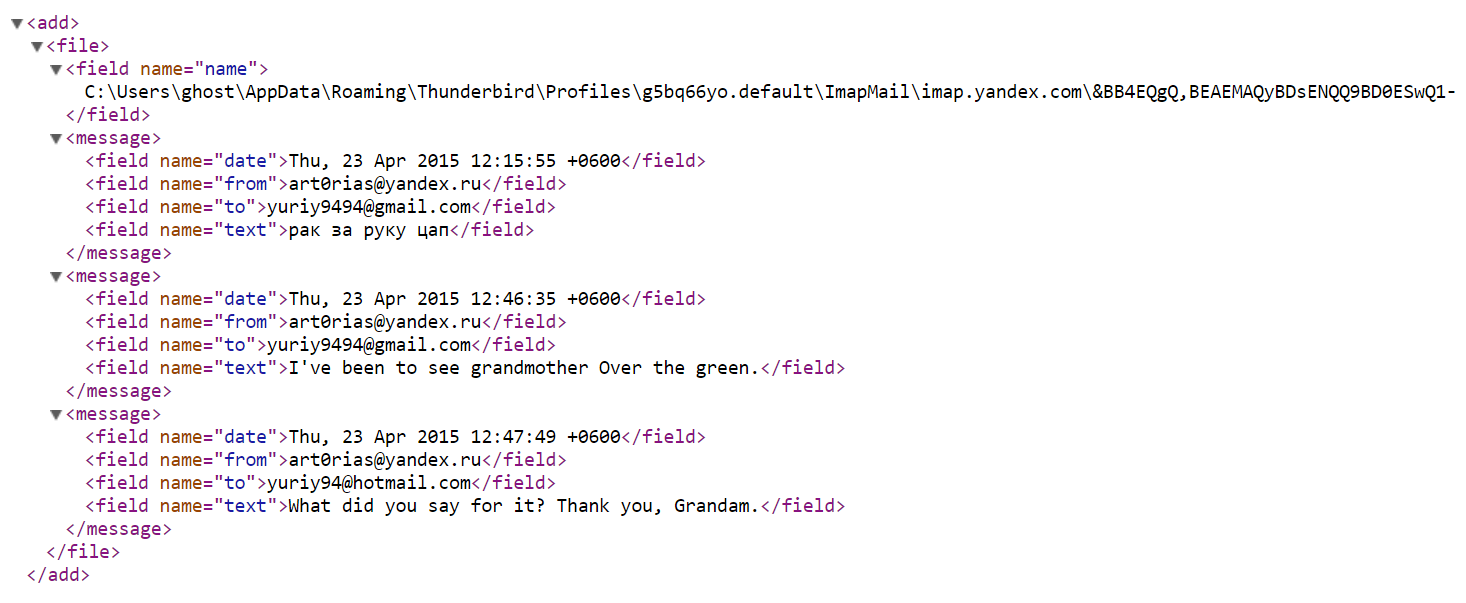
\includegraphics[width=0.9\linewidth]{teresh_2}}
\caption{Пример XML-файла}
\label{teresh_2:teresh_2}
\end{figure}


\newpage
\subsection{Поиск медиа-файлов и извлечение мета-данных} % - Отчет Ильи
Целью работы в текущем семестре было написание программного модуля для нахождения медиа-файлов (аудио, видео, изображение) и извлечения мета-данных.

\subsubsection{Введение}

На базе модуля, сканирующего изображения, была построена основа данного модуля. А именно --- проход по файлам с нужным расширением, считывание базовой информации о файле и вывод в XML формат.

Далее необходимо было изучить структуру мета-данных в медиа-файлах и возможность извлекать эти данные. В качестве начальных форматов тэгов были выбраны ID3v1, JFIF и RIFF. Эти типы мета-данных принадлежат к аудио, изображениям и видео соответственно.

Самым простым в реализации оказался тип ID3v1, с которого и было начато исследование.

\subsubsection{ID3v1}

ID3v1 --- формат метаданных, наиболее часто используемый в звуковых файлах в формате MP3. Он содержит данные о названии трека, альбома, имени исполнителя и годе выпуска. Сами эти данные располагаются в конце файла MP3 и имеют структуру, представленную в таблице~\ref{tab:id3v1}).

Блок-схема алгоритма считывания ID3v1 представлена на рисунке~\ref{bokov_1:bokov_1}. Как следствие, в XML-файле теперь эти данные имеют следующее представление (рис.~\ref{bokov_2:bokov_2}).

\begin{table}[ht]
\caption{Структура ID3v1}
\label{tab:id3v1}
\begin{center}
\begin{tabularx}{\linewidth}{|l|X|}
\hline
Поле & Размер (в байтах) \\
\hline
Заголовок & 3 (всегда равен <<TAG>>) \\
\hline
Название трека & 30 \\
\hline
Имя исполнителя & 30 \\
\hline
Название альбома & 30 \\
\hline
Год выпуска & 4 \\
\hline
Комментарии & 30 \\
\hline
Жанр & 1 \\
\hline
\end{tabularx}
\end{center}
\end{table}

\begin{figure}[h!]
\center{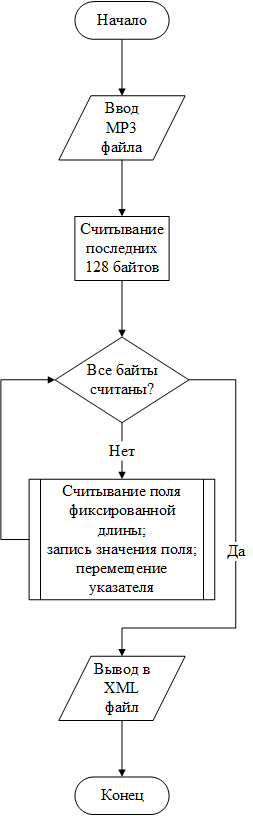
\includegraphics[width=0.3\linewidth]{bokov_1}}
\caption{Блок-схема алгоритма считывания ID3v1}
\label{bokov_1:bokov_1}
\end{figure} 

\begin{figure}[h!]
\center{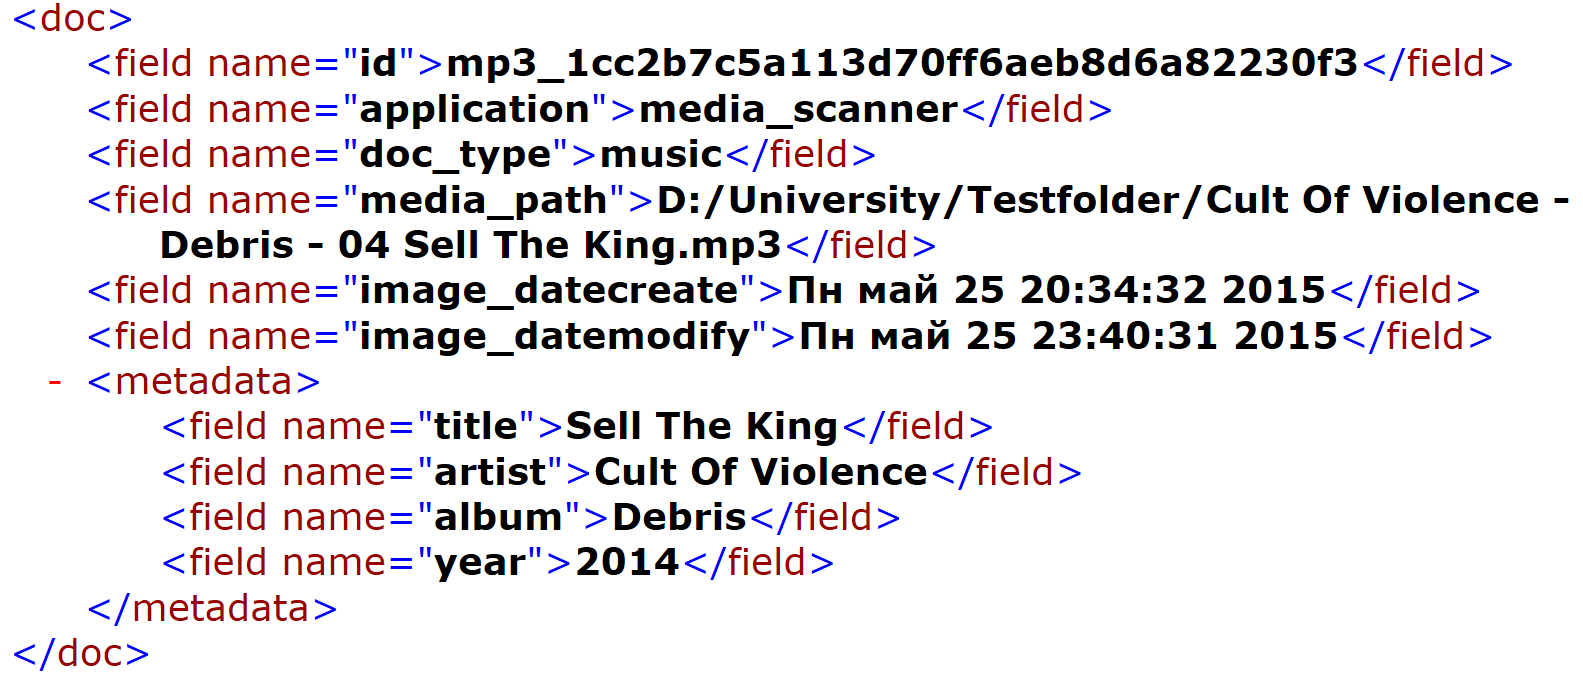
\includegraphics[width=0.6\linewidth]{bokov_2}}
\caption{Результат вывода в XML-файл}
\label{bokov_2:bokov_2}
\end{figure}

\clearpage

\subsubsection{JFIF}

JPEG File Interchange Format (JFIF) --- формат файлов-изображений. Является несколько менее совершенной версией формата EXIF, однако так же позволяет хранить данные об изображении, такие как разрешение изображения, плотность пикселей и данные о миниатюре изображения. Формат представлен в следующем виде ( ~\ref{tab:jfif}).


Блок-схема алгоритма считывания JFIF представлена на рисунке~\ref{bokov_3:bokov_3}, полученный результат в XML-формате --- на рисунке~\ref{bokov_4:bokov_4}.

\begin{table}[ht]
\caption{Структура JFIF}
\label{tab:jfif}
\begin{center}
\begin{tabularx}{\linewidth}{|l|X|}
\hline
Поле & Размер (в байтах) \\
\hline
Маркер APP0 & 2 \\
\hline
Длина & 2 \\
\hline
Идентификатор & 5 \\
\hline
Версия & 2 \\
\hline
Единица измерения плотности & 1 \\
\hline
Плотность по X & 2 \\
\hline
Плотность по Y & 2 \\
\hline
Ширина миниатюры (tw) & 1 \\
\hline
Высота миниатюры (th) & 1 \\
\hline
Данные миниатюры & 3 * tw * th \\
\hline
\end{tabularx}
\end{center}
\end{table}

\begin{figure}[h!]
\center{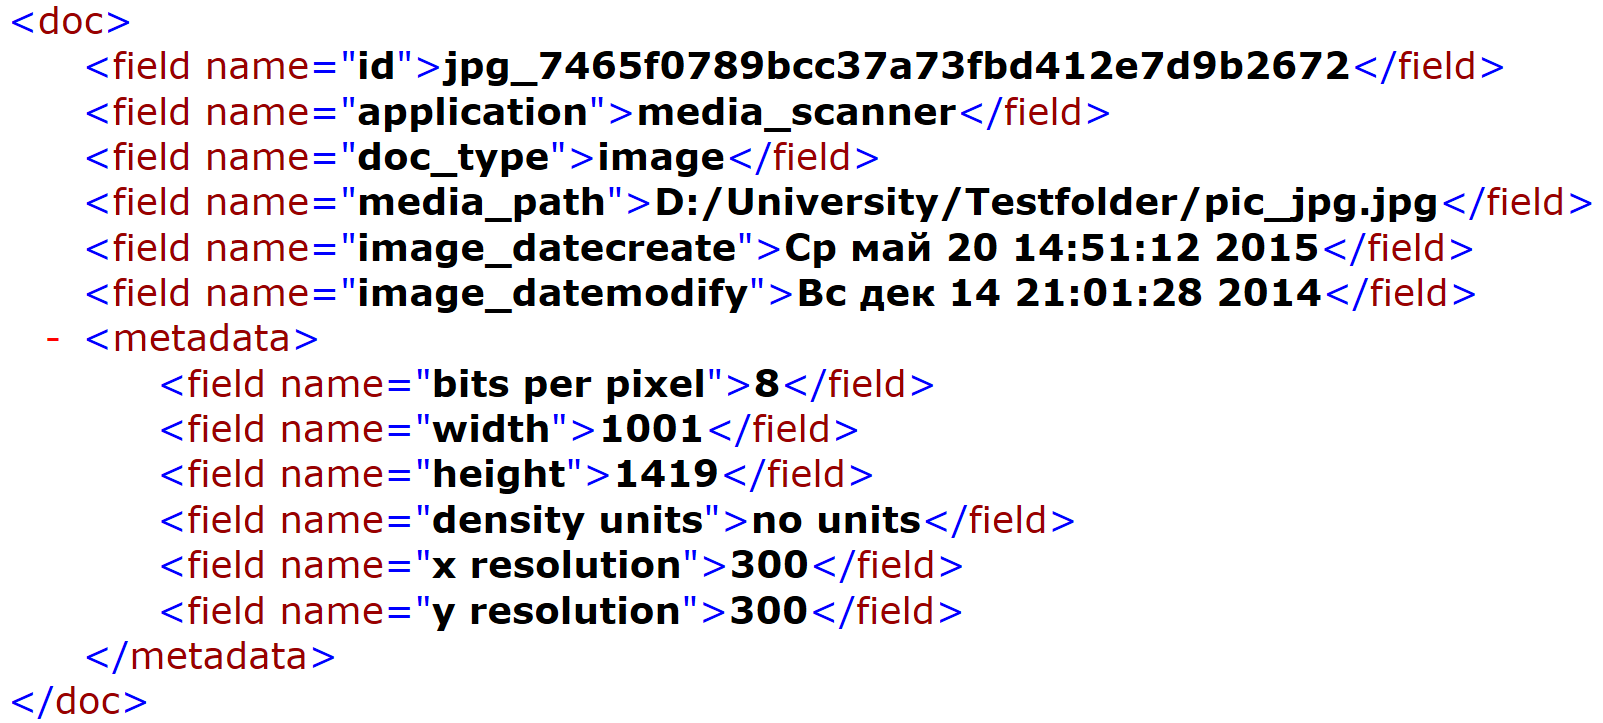
\includegraphics[width=0.7\linewidth]{bokov_4}}
\caption{JPG в XML}
\label{bokov_4:bokov_4}
\end{figure}

\begin{figure}[h!]
\center{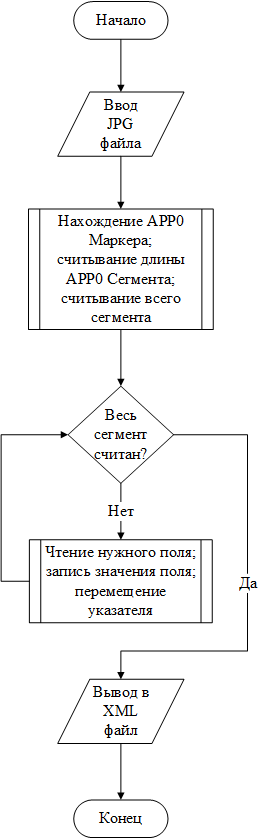
\includegraphics[width=0.4\linewidth]{bokov_3}}
\caption{Считывание JFIF}
\label{bokov_3:bokov_3}
\end{figure} 

\clearpage

\subsubsection{RIFF}

Resource Interchange File Format (RIFF) --- один из форматов файлов-контейнеров для хранения потоковых мультимедиа-данных. Наиболее известными форматами, использующими RIFF в качестве контейнера, является AVI.
Основной концепцией формата является chunk -- порция данных с заголовком и сигнатурой, указывающей на содержимое chunk`а.
В chunk`е strh хранятся общие данные о потоке и определение того, какого типа этот поток (аудио, видео, текст или midi). Соответственно, в его дочернем chunk`е (strf) содержится следующая информация, если это видео (таблица~\ref{tab:strf}).

\begin{table}[ht]
\caption{Структура strf (vids)}
\label{tab:strf}
\begin{center}
\begin{tabularx}{\linewidth}{|l|X|}
\hline
Номер байта & Метаданные \\
\hline
0-3 & STRF \\
\hline
4-7 & Размер \\
\hline
8-11 & Ширина \\
\hline
12-15 & Высота \\
\hline
16-19 & Bit planes \\
\hline
20-23 & Кол-во бит на пиксель \\
\hline
24-27 & Сжатие бит \\
\hline
28-31 & Размер изображения \\
\hline
32-35 & Горизонтальное разрешение \\
\hline
36-39 & Вертикальное разрешение \\
\hline
40-43 & Показатель цвета \\
\hline
44-49 & Количество важных цветов \\
\hline
\end{tabularx}
\end{center}
\end{table}

Если же это аудио, то информация будет выглядеть следующим образом (таблица~\ref{tab:auds}).

\begin{table}[ht]
\caption{Структура strf(auds)}
\label{tab:auds}
\begin{center}
\begin{tabularx}{\linewidth}{|l|X|}
\hline
Номер байта & Метаданные \\
\hline
0-3 & STRF \\
\hline
4-7 & Размер \\
\hline
8-9 & Компрессор \\
\hline
10-11 & Каналы \\
\hline
12-13 & Частота дискретизации \\
\hline
14-15 & Байты в секунду \\
\hline
16-17 & Block align \\
\hline
18-19 & Бит на семпл \\
\hline
\end{tabularx}
\end{center}
\end{table}

Алгоритм обработки RIFF --- рисунок~\ref{bokov_5:bokov_5}, вывод в XML-файл --- рисунок~\ref{bokov_6:bokov_6}. 

\begin{figure}[h!]
\center{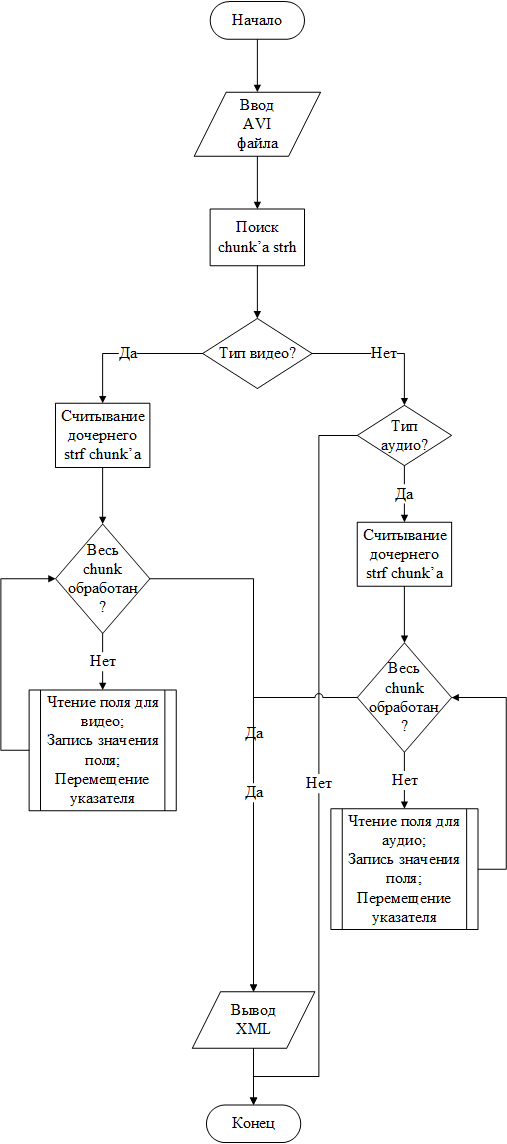
\includegraphics[width=0.5\linewidth]{bokov_5}}
\caption{Алгоритм обработки RIFF}
\label{bokov_5:bokov_5}
\end{figure} 

\begin{figure}[h!]
\center{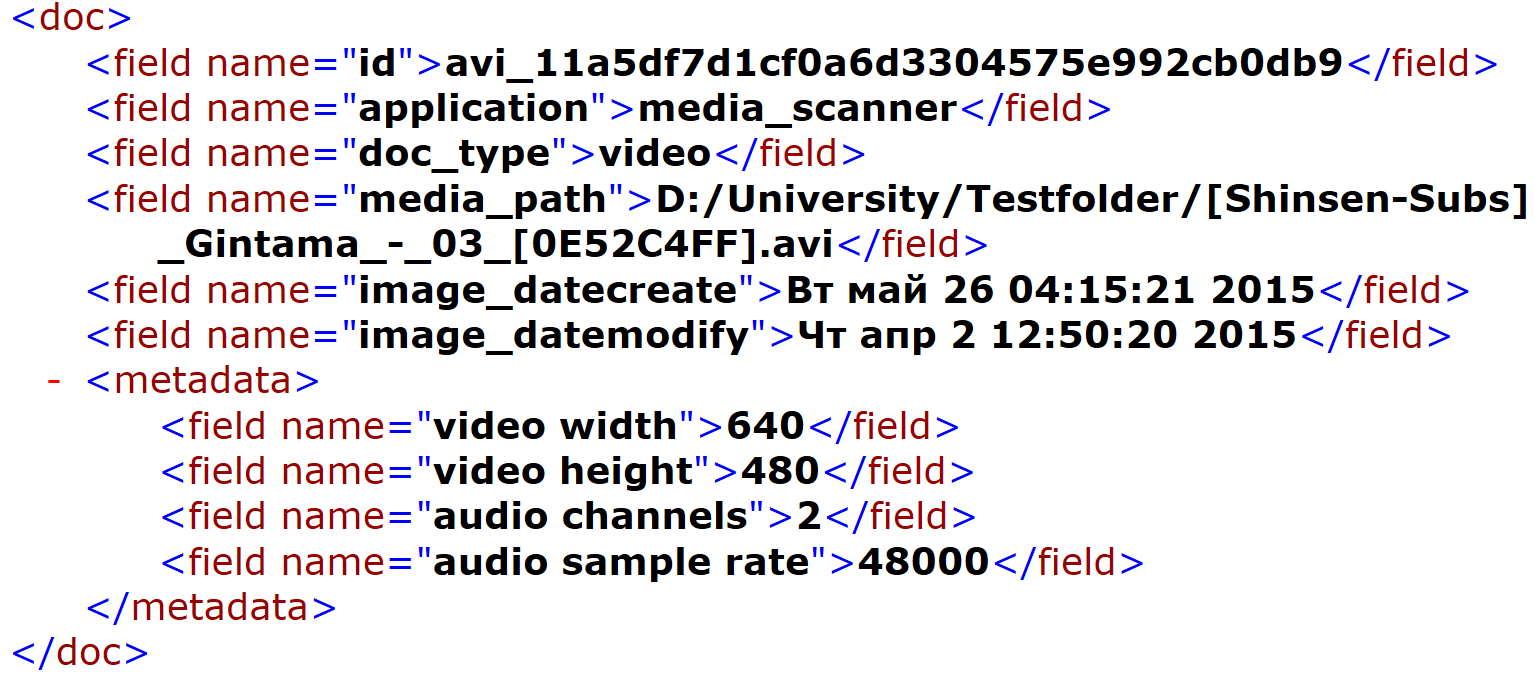
\includegraphics[width=0.4\linewidth]{bokov_6}}
\caption{Результат в XML}
\label{bokov_6:bokov_6}
\end{figure}

\subsubsection{Задачи на следующий семестр}

На данный момент программа является модульной, что позволяет без особого труда добавлять в нее поддержку новых расширений и типов форматов мета-данных. В будущем планируется добавление таких форматов мета-данных, как mkv, exif, id3v2, и поддержка еще большего количества расширений, а также усовершенствование работы программы с уже имеющимися форматами.

В этом семестре реализовано:

\begin{itemize}
  \item рекурсивный обход директорий;
  \item чтение формата мета-данных для видео RIFF;
  \item чтение полей тегов формата JFIF;
  \item чтение информации об mp3 из контейнера ID3v1.
\end{itemize}

\clearpage


\newpage 
\subsection{Сбор и анализ информации из реестра ОС MS Windows} % - Отчет Олега
Одним из этапов проведения компьютерной экспертизы является анализ установленного программного обеспечения. Общеизвестно, что наличие единого реестра в системе, стало одной из особенностей операционной систем семейства Windows. В большинстве случаев, программы используют его в качестве хранения каких-либо данных.

Реестр Windows представляет собой иерархически построенную базу данных. На этапе загрузки операционная система собирает его из <<исходных>> файлов, разбросанных по своему дистрибутиву.

Целью работы за этот семестр стояло извлечь полезную информацию из реестра Windows, для достижения которой были выделены следующие задачи:

\begin{enumerate}
  \item исследовать механизм формирования реестра;
  \item написание программного модуля, способного извлекать информацию из реестра.
\end{enumerate}

\subsubsection{Исследование механизма формирования реестра}

Семестром ранее был установлен список исходных файлов реестра и было проведено первое знакомство с их структурой.

В ходе исследования одного из файлов было установлено, что он представляет собой <<чистый>> байтовый массив данных (рис.~\ref{lob_1:lob_1}). Встал вопрос о структуре данных в нем.

Компания Microsoft разрабатывает операционную систему Windows с конца прошлого века и, несмотря на <<закрытость>> исходного кода, время от времени выкладывает код отдельных ее модулей. \cite{registry} К сожалению, к ним не относится модуль реестра.

Из альтернативных источников можно получить лишь приблизительное представление внутренней структуре (рис.~\ref{lob_2:lob_2}). \cite{msdn}

К сожалению, из-за недостатка информации, придется на время отказаться от идеи разбора <<сырых>> файлов.

\begin{figure}[h!]
\center{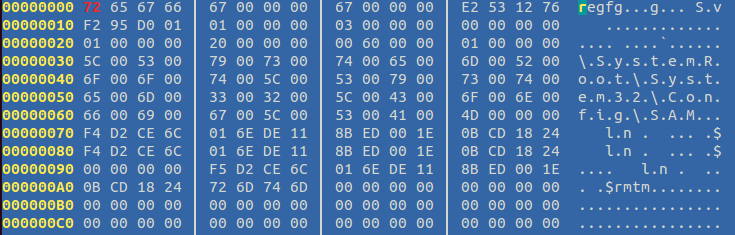
\includegraphics[width=0.9\linewidth]{lob_1}}
\caption{Файл SAM в HEX редакторе}
\label{lob_1:lob_1}
\end{figure} 

\begin{figure}[h!]
\center{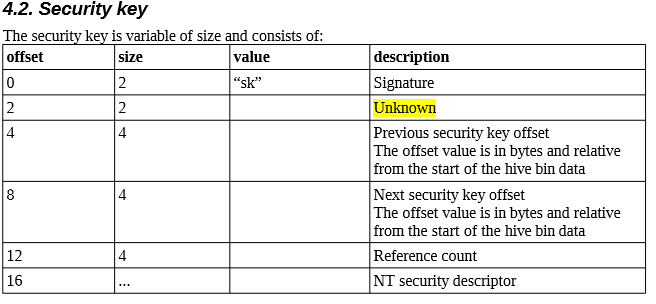
\includegraphics[width=0.9\linewidth]{lob_2}}
\caption{Пример описания одного из «простейших» блоков данных}
\label{lob_2:lob_2}
\end{figure} 

\subsubsection{Написание программного модуля, способного извлекать информацию из реестра}

С помощью встроенной в Windows утилиты regedit был сделан дамп всего древа реестра. Дальнейшая работа будет вестись с этим дампом.

Файл представляет из себя строковый массив с данными 2-х видов:

\begin{enumerate}
  \item описание ветви: [путь\_через\_узлы];
  \item описание данных: <<название поля>> = значение.
\end{enumerate}



\begin{figure}[h!]
\center{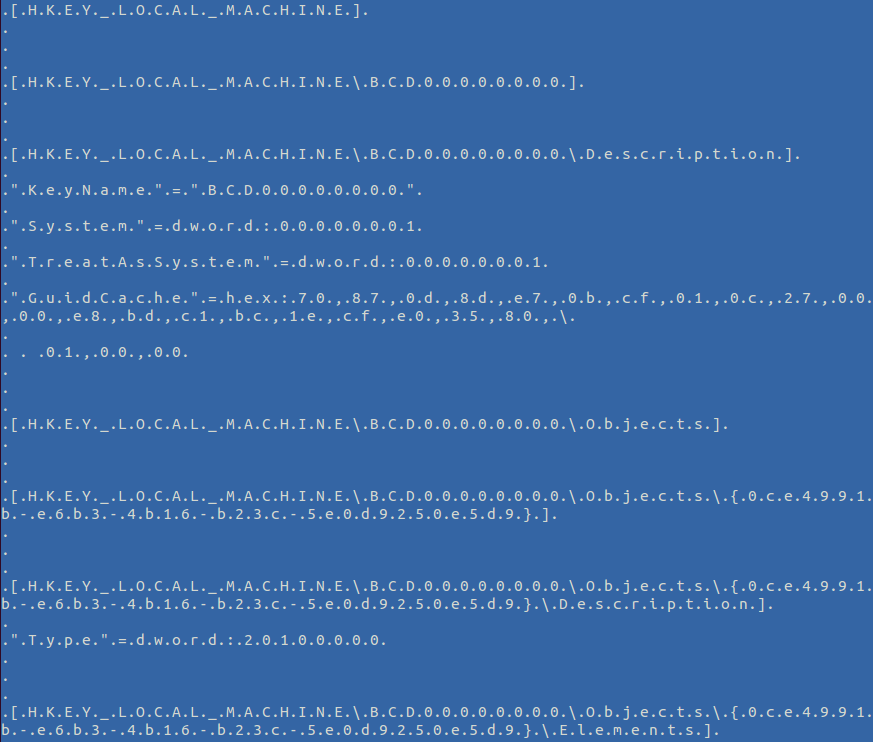
\includegraphics[width=0.9\linewidth]{lob_3}}
\caption{Внутренности .reg файла}
\label{lob_3:lob_3}
\end{figure} 

\begin{figure}[h!]
\center{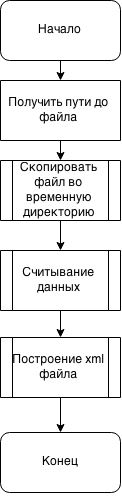
\includegraphics[width=0.2\linewidth]{lob_4}}
\caption{Блок-схема алгоритма работы модуля}
\label{lob_4:lob_4}
\end{figure} 

Считывание данных происходит построчно, рассмотрим в общем виде, как оно должно проходить (рис.~\ref{lob_5:lob_5}).

Пример работы программы представлен на рисунке~\ref{lob_6:lob_6}, результат работы программы --- на рисунке~\ref{lob_7:lob_7}.

\begin{figure}[h!]
\center{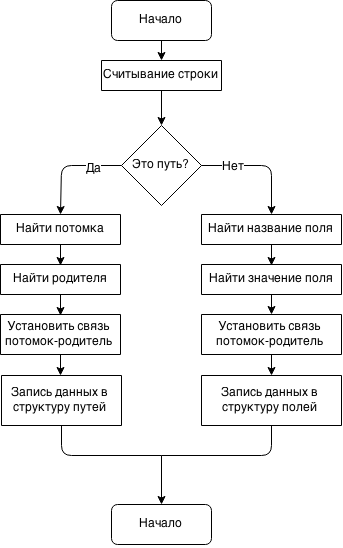
\includegraphics[width=0.4\linewidth]{lob_5}}
\caption{Функция разбора одной строки}
\label{lob_5:lob_5}
\end{figure} 

\begin{figure}[h!]
\center{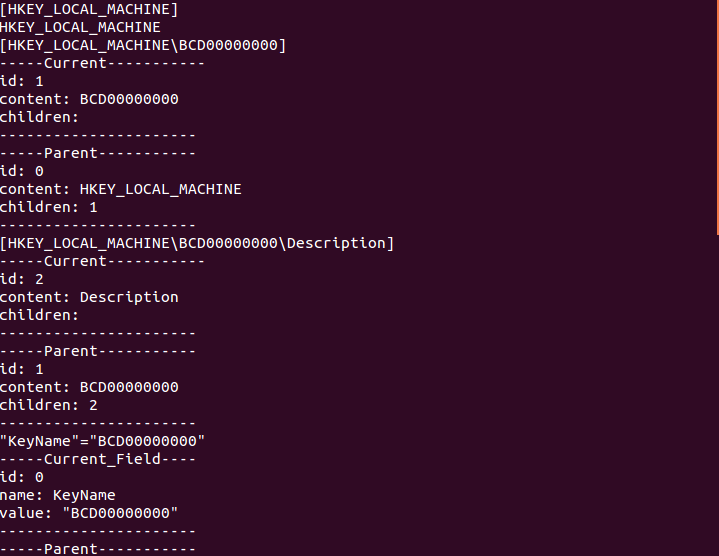
\includegraphics[width=0.7\linewidth]{lob_6}}
\caption{Пример работы программы}
\label{lob_6:lob_6}
\end{figure} 

\begin{figure}[h!]
\center{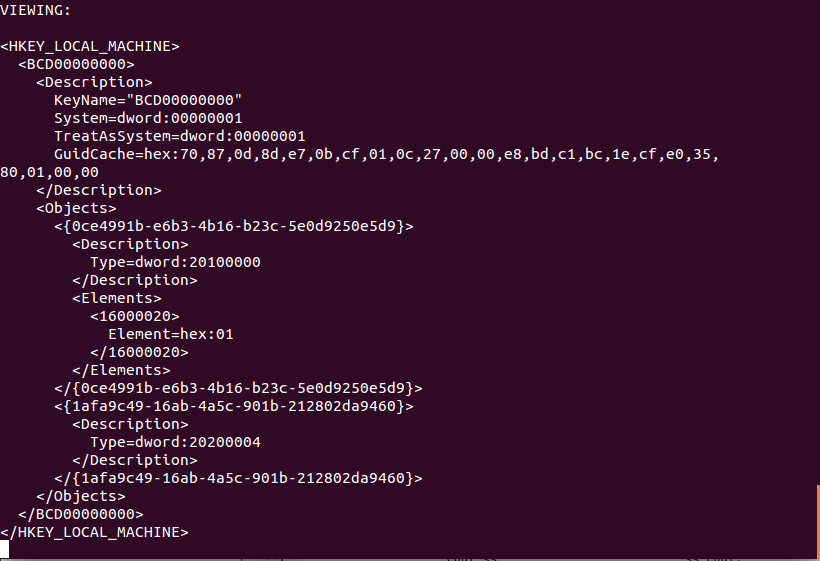
\includegraphics[width=0.7\linewidth]{lob_7}}
\caption{Результат работы программы}
\label{lob_7:lob_7}
\end{figure} 

\subsubsection{Результаты работы за семестр}

Результаты работы за текущий семестр:

\begin{enumerate}
  \item проведено доисследование структуры исходных файлов реестра;
  \item написан модуль получения информации из реестра windows. Информация берется из .reg файлов.
\end{enumerate}

Планы на будущее:

\begin{enumerate}
  \item дальнейший поиск описаний структура исходных файлов;
  \item по возможности, написание модуля извлечения информации из этих файлов.
\end{enumerate}

\clearpage








\newpage
\section*{Заключение}
\addcontentsline{toc}{section}{Заключение}
В данном семестре нашей группой была выполнена часть работы по созданию автоматизированного программного комплекса для проведения компьютерной экспертизы, проанализированы дальнейшие перспективы и поставлены цели для дальнейшего развития проекта.
 
 
 \newpage
 \renewcommand{\refname}{Список использованных источников}
 \bibliography{lit}

 \ESKDappendix{Обязательное}{\normalfont Компакт-диск}
 Компакт-диск содержит: 
 \begin{itemize}
 \item электронную версию пояснительной записки в форматах *.tex и *.pdf;
 \item актуальную версию программного комплекса для проведения компьютерной экспертизы;
 \item тестовые данные для работы с программным комплексом;
 \item документацию к проекту в html-формате.
 \end{itemize}
 
\end{document}
